\documentclass[11pt]{book}
\usepackage{amsmath,amssymb,amsfonts,amsthm}
\usepackage{tikz}
\usepackage{braket}
\usepackage{iiit_thesis}
\usepackage{cite}
\usepackage{times}
\usepackage{graphicx}
\usepackage{setspace}
\usepackage{enumitem}
\usepackage{tabularx}
\usepackage{subfigure}
\usepackage{notoccite}
\usepackage{afterpage}
\usepackage{xcolor}
\usepackage{algorithm}
\usepackage{algpseudocode}
\usepackage{multirow}
\usepackage[hidelinks]{hyperref} 
\usepackage[toc,page]{appendix}
\usepackage{comment}
\usepackage{pdfpages}
\usepackage{siunitx}
\newtheorem{prop}{Proposition}
\newtheorem{theorem}{Theorem}
\newtheorem{result}{Result}

\graphicspath{{images/}{./}} % To include images in other directories

%------------------------------------------------
% To reduce separation in itemize and enumerate
% \setlist[itemize]{noitemsep} % can include 'nolistsep' also
% \setlist[enumerate]{noitemsep}

%------------------------------------------------
% Settings for Abbreviations and Symbols list
\usepackage[style=super,automake,nogroupskip,nopostdot,symbols,sort=standard,toc=false]{glossaries-extra}
\setglossarystyle{super}
\setabbreviationstyle[acronym]{long-short}
  % \centering
  \renewenvironment{theglossary}%
    {\tablehead{}\tabletail{}%
     \begin{supertabular}{p{4cm}p{\glsdescwidth}}}%
    {\end{supertabular}}%
\makeglossaries

%-------------------------------------------------
\long\def\symbolfootnote[#1]#2{\begingroup%
\def\thefootnote{\fnsymbol{footnote}}\footnote[#1]{#2}\endgroup}
\renewcommand{\baselinestretch}{1.2}
\onecolumn
%
\makeatletter
\def\ignorecitefornumbering#1{%
     \begingroup
         \@fileswfalse
         #1%                     % do \cite comand
    \endgroup
}
\makeatother

%-------------------------------------------------
% Custom commands
\newcommand{\p}{\mathbb{P}}
\newcommand{\gt}{\gamma_{\text{th}}}
\newcommand\txtblue[1]{{\color{blue}#1}}
%\newcommand{\ket}{}
%--------------------------------------------------------

\begin{document}
\pagenumbering{roman}
%% TITLE PAGE
\thispagestyle{empty}
\begin{center}
\vspace*{1.5cm}
{\Large \bf Quantum Switch and it's applications in Quantum Information Theory}

\vspace*{2.2cm}
{\large A thesis submitted in partial fulfillment\\}
{\large  of the requirements for the degree of \\}

\vspace*{1cm}
{\it {\large Masters by Research } \\
{\large in\\}
{\large Computer Science Engineering \\}}

\vspace*{0.8cm}
{\large by}

\vspace*{6mm}
{\large Sravani Yanamandra\\}
{\large 2021701022\\
{\small \tt sravani.yanamandra@research.iiit.ac.in}}

\vspace*{5mm}
{\large Advisor: Dr. Samyadeb Bhattacharya\\}


\vspace*{3.0cm}
{
\includegraphics[width=5cm]{figures/iiit.png}\\}
{\large International Institute of Information Technology Hyderabad\\}
{\large 500 032, India\\}
\vspace*{5mm}
{\large March 2024\\}
\end{center}

%----------COPYRIGHT PAGE--------------------
\newpage
\thispagestyle{empty}
\renewcommand{\thesisdedication}{{\large Copyright \copyright~Sravani Yanamandra, 2024\\}{\large All Rights Reserved\\}}
\thesisdedicationpage

%------------------------------------------------
\newpage
\thispagestyle{empty}
\vspace*{1.5cm}
\begin{center}
{\Large International Institute of Information Technology Hyderabad\\}
{\Large Hyderabad, India\\}
\vspace*{3cm}
{\Large \bf CERTIFICATE\\}
\vspace*{1cm}
\noindent
\end{center}
This is to certify that work presented in this thesis proposal titled \textit{\textbf{Absolute Separability and Quantum Switch}} by \textit{Sravani Yanamandra} has been carried out under my supervision and is not submitted elsewhere for a degree.

\vspace*{3cm}
\begin{tabular}{cc}
\underline{\makebox[1in]{}} & \hspace*{5cm} \underline{\makebox[2.5in]{}} \\
Date & \hspace*{5cm} Advisor: Dr. Samyadeb Bhattacharya
\end{tabular}
\mastersthesis
% \renewcommand{\baselinestretch}{1.5}
%
% ABSTRACT PAGE
\chapter*{Abstract}
\label{ch:abstract}
    Absolute separable (AS) quantum states are those states from which it is impossible to create entanglement, even under global unitary operations. It is known from the resource theory of non-absolute separability that the set of absolute separable states forms a convex and compact set, and global unitaries are free operations. We show that the action of a quantum switch controlled by an ancilla qubit over the global unitaries can break this robustness of AS states and produce ordinary separable states. First, we consider bipartite qubit systems and find the effect of quantum switch starting from the states sitting on the boundary of the set of absolute separable states. As particular examples, we illustrate what happens to modified Werner states and Bell diagonal (BD) states. For the Bell diagonal states, we provide the structure for the set of AS BD  states and show how the structure changes under the influence of a switch. Further, we consider numerical generalization of the global unitary operations and show that it is always possible to take AS states out of the convex set under switching operations. We also generalized our results in higher dimensions.
%
\tableofcontents
%\listoffigures
%\let\cleardoublepage\clearpage
%\listoftables
%\printglossary[type=\acronymtype,title=Abbreviations,nonumberlist]
%\printunsrtglossary[type=symbols]

%--------------------------------------------------------
% 'List of Publications'
\chapter*{List of Related Publications}
\label{ch:relatedPubs}
\begin{enumerate}[label={[P\arabic*]}]  
    \item S. Yanamandra, P. V. Srinidhi, S. Bhattacharya, I. Chakrabarty, and S. Goswami,\textbf{“Breaking absolute separability with quantum switch"}, 2023.
\end{enumerate}
\noindent
Related co-author publications:
\begin{enumerate}[start=2,label={[P\arabic*]}]
    \item S. Mukharjee, B. Mallick, S. Yanamandra, S. Bhattacharya and A.G. Maity, \textbf{“Interplay between the Hilbert-space dimension of the control system and the memory induced by quantum SWITCH”}, Oct 2023
\end{enumerate}

%--------------------------------------------------------
\chapter{Introduction}
\label{ch:intro}
In 1935, Einstein, Podolsky, and Rosen (EPR) first pointed out the concept of non-local effect in quantum systems in terms of a paradox \cite{EPR_35}. Later in the same year, while trying to explain the paradox, Schr\"{o}dinger \cite{S_35} introduced the term ``entanglement'' and the concept of quantum steering \cite{S_35, WJD_07, JWD_07} which eventually leads to another quantum correlation i.e. Bell-nonlocality \cite{B_64}. From then on, in the literature of quantum information theory, the concept of entanglement as a quantum correlation has consistently been the most dominant one. It is not only of philosophical interest where it deals with deep concepts like realism and locality but also acts as a cardinal resource in various information processing tasks such as teleportation \cite{BBCJPW_93}, super dense coding \cite{BW_92} and many more \cite{BB_84, E_91}. In the recent developments in quantum computation, entanglement is an intricate resource for speed-ups compared to the corresponding classical counterparts \cite{LP_01, JL_03,V_13,GH_23} and also to minimize the effect of environmental noise \cite{DGPM_17}. When multipartite systems are considered, entanglement is one of the most basic forms of non-classical correlation that is also a resource. On the other hand, quantum steering is a stronger form of correlation than entanglement and the steerable states form a strict subset of entangled states. Finally, the Bell non-local states are a strict subset of steerable states. This hierarchy \cite{WJD_07} and application of all these non-local correlations are well explored in literature \cite{TR_11,BCWSW_12}. \\\\
Entangled states are those which are not separable in nature i.e. they can not be written as a convex mixture of product states of the corresponding subsystems. From the perspective of entanglement resource theory \cite{HHH_09}, the local operations and classical communication (LOCC) are the free operations, using which neither entanglement can be created from a separable state, nor can be increased. Hence in this resource theory, the separable states are the free states and they form a convex and compact set.Defining separability of a given mixed state $\rho$, we implicitly assume that the product structure of the composite
Hilbert space is given, $\mathcal{H} = \mathcal{H}_A \otimes \mathcal{H}_B$. This assumption is well justified from the physical point of view. For example,
the EPR scenario distinguishes both subsystems in a natural way. Then we speak about separable (entangled) states, with respect to this particular decomposition of $\mathcal{H}$. Note that any separable pure state may be considered entangled, if analyzed with respect to another decomposition of $\mathcal{H}$.
On the other hand, one may pose a complementary question, interesting merely from the mathematical point of view, which states are separable with respect to any possible decomposition of the $\mathcal{N} = \mathcal{K} \text{ x } \mathcal{M}$ dimensional Hilbert space $\mathcal{H}$. Now it is natural to ask if one has free access to global operations, then is it possible to create entanglement from a separable state? The answer is in general affirmative but is not always true. There is a set of states which is so strongly separable that it is not possible to generate entangled states from them via any global unitary or even via the convex combination of them \cite{KZ_01, VAD_01, KC_01, LHL_03}. These states are called absolute separable (AS) states. Recently, in \cite{PMD_22} the resource theory of non-absolute separability is introduced where global unitaries are the free operations and the non-AS states are the resourceful states. 
%\textcolor{blue}{Absolute local and other references are missing Ref: https://link.springer.com/article/10.1007/s11128-017-1734-4,\\ https://www.worldscientific.com\\/doi/abs/10.1142/S0219749918500405}\\
In this work, we try to connect the effect of indefinite causal order along with post-selection with the possibility of generating some resourceful state starting from AS states using global unitary operations. From the resource theoretic point of view, if we have global unitary operations for free, then can we take states out of the convex set of AS states? We answer the question affirmatively with the help of a quantum switch. Here, we consider that the two global unitary operations represented by two channels $(\mathcal{N}_1, \mathcal{N}_2)$ are acting sequentially. The power of switching is induced by introducing the ancillary system, which dictates that with some probability $\mathcal{N}_2$ acts after $\mathcal{N}_1$ and $\mathcal{N}_1$ acts after $\mathcal{N}_2$ with rest of the probability. Next, to ensure the effect of indefinite causal ordering, we consider the superposition of these two scenarios. Finally a post-selection is done by performing a projective measurement on the ancillary system. The overall effect of the switching action hence consists of the superposition of the global unitaries followed by the post-selection. In the beginning, we consider AS states lying on the boundary of the convex set and show that by using global unitary with switching action, one can take these states out of this set. Next, we consider two-qubit modified Werner state and show how the range of the AS states changes with the value of the parameters in the presence of quantum switch. We notice that it is possible to make even a maximally mixed state resourceful by using the switching operation of suitably chosen unitary. In \cite{LC_10}, the authors identify the geometry of the separable BD states. Here, we extend the results for AS states and show how the structure changes in the presence of switching on global unitary operations. Additionally, we generalize our results numerically by Haar uniformly generating random global unitary matrices. We show our protocol is effective even in higher dimensions.

\section{Motivation}
Quantum switch is a circuit that implements indefinite causal order among a set
of quantum operations (We refer the readers to \cite{OCB_12} for a detailed discussion
on indefinite causal order) \cite{chiribella_2009}. The experimental demonstration of the quantum
switch has been reported in \cite{PMACADHRBW_15},\cite{RRFAZPBW_17}. There exist several applications of the
quantum switch in different information - theoretic/communication tasks. Some of
these applications, we mention below. In \cite{mukhopadhyay_2020},\cite{8966996}, the quantum switch has
been applied in quantum teleportation. In \cite{ESC_18},\cite{PhysRevA.103.062610}, it has been shown that
using quantum switch, the transmission of classical information is possible through
quantum channels that have the maximally mixed state as a fixed output. It has been
shown in \cite{CBBGARSAK_21} that even perfect quantum communication can be achieved using
an entanglement breaking channel using the quantum switch. In \cite{procopio_2019}, quantum
switch has been used on N quantum channels to enhance classical communication.
Quantum switch also has been used to test the properties of quantum channels
\cite{PhysRevA.86.040301},\cite{ACB_14}. In \cite{PhysRevLett.124.190503}, it has been discussed that the quantum switch can be used
to boost the precision of quantum metrology. Quantum switch has been also used
to reduce quantum communication complexity \cite{GFAC_16}. There may be more possible
applications of the quantum switch that are yet to be studied. A part of this thesis
is based on improvement in quantum communication using quantum switch.\\\\
In the recent past, the literature of quantum information theory evidently illustrates that indefinite ordering of multiple causal events can give rise to advantages in terms of resource requirements in different quantum protocols. The concept of indefinite causal ordering was first pointed out in \cite{H_05, H_07} and was extended to resource theoretic frameworks in \cite{CDPV_13}. Exploiting this concept, the structure of quantum switch was introduced \cite{CDPV_13}, where we essentially consider an ancillary system that acts as a controller to the orders of the events. A stronger approach to this indefiniteness is by process matrix formalism introduced in \cite{OCB_12}. Indefinite causal ordering has played a significant role in increasing the efficacy of various information processing activities. These include winning non-local games \cite{OCB_12}, testing properties of quantum channel \cite{C_12}, minimizing quantum communication complexity \cite{GFAC_16}, improving quantum communication \cite{ESC_18, CBBGARSAK_21,Mitra_2023}, increasing the performance of quantum algorithm \cite{ACB_14}, activating non-Markovianity \cite{MB_22,agm_23} and many more. Recent developments in this domain are centered around providing experimental evidence \cite{PMACADHRBW_15, RRFAZPBW_17, GGKCBRW_18}. 

\section{Outline}
The rest of the thesis is organized as follows. In Chapter 2, we discuss the preliminaries that are required for the later parts of the thesis. In Chapter 3, the concepts of Open Quantum Systems and their standard equation are described. Chapter 4 is based on the topic of Indefinite Causal Order and their applications. In Chapter 5, we explain the work done in the paper \cite{yanamandra2023breaking}. We conclude the work and it's results in chapter 6.

%--------------------------------------------------------
\chapter{Preliminaries}
\label{ch:ch1}

\subsection{Schmidt Decomposition:}
 let $\ket{\phi}$ be a state in a Hilbert space $\mathcal{H}$, then the Schmidt rank of the state written in Schmidt decomposition $\ket{\phi}=\sum_j \alpha_j \ket{j^A} \ket{j^B}$ is the number of nonzero $\alpha_j$ parameters. Let $\ket{\phi}$ be a state, the Schmidt rank of the state is denoted by rk($\ket{\phi}$).
\subsection{Mixed States}
It is not always known what exact pure state is occupied by a given
quantum system. In this case, all that is known is the set of possible pure states and probabilities of the pure states occurring. Therefore, it is important to consider classically probabilistic distribution
amongst the pure states. This distribution gives rise to the set of
mixed states.\\
Let $\{\phi_i\}_{i=1}^k$ be a set of pure states in a Hilbert space $\mathcal{H}$, then any convex combination of the pure states yields a mixed state. The mixed states are represented by convex combinations of the outer products of pure states known as density matrices.
\begin{equation}
    \rho=\sum_{i=1}^k p_i \ket{\phi_i}\bra{\phi_i} \text{ where } p_i \geq 0 \text{ and } \sum_{i=1}^k p_i = 1
\end{equation}
From the duality of matrices and linear operators, it follows that
the mixed states are linear operators and hence, the term density operator is often used to refer to a mixed state. From the definition of
mixed states, it immediately follows that all pure states are mixed.
However, the converse does not hold. In fact, the statement can be
further generalised to the following theorem showing the relation
between the set of mixed states and the set of pure states. A mixed state $\rho$ is a pure state if and only if there is a single
pure state in the convex combination of the mixed state $\rho$. Therefore, we end up with the statement that pure states are extremal points of the convex set. 

\subsection{Trace}
The trace of $O$ is a map $\mathrm{Tr}:\mathcal{L}(\mathcal{H})\rightarrow\mathbb{C}$
defined as the sum of the diagonal elements of $O$ when it is represented
in a certain basis $|\psi_{j}\rangle\in\mathcal{H}$, i.e., $\mathrm{Tr}(O)=\sum_{j=1}^{d}\langle\psi_{j}|O|\psi_{j}\rangle,$
with $d$ being the dimension of $\mathcal{H}$.
The trace of a density matrix representation of a pure state is related to its inner product as it holds that $Tr(\ket{\phi}\bra{\phi}) = \braket{\phi}{\phi}$ = 1. The trace can also help determine whether a given density matrix $\rho$ is a matrix for a pure state or a mixed state. It suffices to compute
the trace of the square of density matrix as it holds for all density
matrices that Tr($\rho^2$) $\leq$ 1 and the trace is equal to 1 if and only if the state is pure.\cite{Arfken}.
It was already discussed that trace of a density matrix representation of a pure state is related to its inner product and hence, it is
always 1. In fact, trace of all mixed states is always 1. Furthermore,
every density matrix of trace 1 corresponds to a mixed state. Therefore, mixed states form a convex set.
\subsection{Partial Trace}
By its turn, in the quantum mechanics of composite systems with Hilbert
space $\mathcal{H}=\mathcal{H}_{a}\otimes\mathcal{H}_{b}$, the \emph{partial
trace function}, taken over sub-system $b$, can be defined as \cite{Watrous}
\begin{equation}
\mathrm{Tr}_{b}(O)=\sum_{j=1}^{d_{b}}(\mathbb{I}_{a}\otimes\langle b_{j}|)O(\mathbb{I}_{a}\otimes|b_{j}\rangle),\label{eq:ptr1}
\end{equation}
with
\begin{equation}
|b_{j}\rangle=[b_{j1}\mbox{ }b_{j2}\mbox{ }\cdots\mbox{ }b_{jd_{b}}]^{t}
\end{equation}
being any orthonormal basis for $\mathcal{H}_{b}$, $\langle b_{j}|=|b_{j}\rangle^{\dagger}$,
$d_{b}=\dim\mathcal{H}_{b}$, and $\mathbb{I}_{b}$ is the identity
operator in $\mathcal{H}_{b}$. So the
partial trace is a map
\begin{equation}
\mathrm{Tr}_{b}:\mathcal{L}(\mathcal{H})\rightarrow\mathcal{L}(\mathcal{H}_{a});
\end{equation}

It is worthwhile observing here that the definition above is equivalent
to \emph{another definition} which appears frequently in the literature
\cite{Nielsen_Chuang_2010}:
\begin{equation}
\mathrm{Tr}_{b}(|a\rangle\langle a'|\otimes|b\rangle\langle b'|)=|a\rangle\langle a'|\otimes\mathrm{Tr}_{b}(|b\rangle\langle b'|).\label{eq:ptr_def2}
\end{equation}

Partial trace is the only function $f:\mathcal{L}(\mathcal{H}_{a}\otimes\mathcal{H}_{b})\rightarrow\mathcal{L}(\mathcal{H}_{a})$
such that $\mathrm{Tr}_{ab}(A\otimes\mathbb{I}_{b}O)=\mathrm{Tr}_{a}(Af(O))$,
for generic linear operators $A\in\mathcal{L}(\mathcal{H}_{a})$ and
$O\in\mathcal{L}(\mathcal{H}_{a}\otimes\mathcal{H}_{b})$ and it holds that 
\begin{equation}
    Tr_{b}(\mathcal{L^A} \otimes \mathcal{L^B}) = \mathcal{L^A}Tr(\mathcal{L^B})
\end{equation}

%--------------------------------------------------------
\label{ch:oqs}
\begin{comment}
    The study on quantum phenomenon is always observed using a closed system. But in reality, the system we live in is in contact with environment and is not exclusive from it. It means that the system is not isolated and the effect of the environment is there on the system. Due to this, it is crucial to develop a theoretical framework to interact and understand the quantum system.When we consider a pure state, there is no unitary evolution implemented on the state to convert it from a pure state to a mixed state. We find that the purity of the state is conserved in a unitary operation. But there are legitimate physical processes that constitute the transition from a pure state to a mixed state.Open quantum system can be defined as a quantum system that is in continuous interaction with the environment(which is also a quantum system).In this report, we study how to better formulate the interactions as these interactions with the environment significantly change the dynamics of the system and result in quantum dissipation.Applying the concepts learnt from open quantum systems, we can better understand the system, develop better tools to add the environment effect into the interaction while evolution occurs, remove the same when focus is needed on the system alone and make the theoretical interactions match the physical counterparts.
\end{comment}
\subsection{Composite Systems:}
    
   To talk about the evolution of open systems, we can consider the system to be a part of a larger closed system that is undergoing a Unitary evolution. This larger closed system consists of a subsystem that is of interest to us, and another subsystem which is the environment. Then, the total system can be denoted as follows:
   \begin{equation}
        \ket{\rho} = \ket{\rho_{system}} \otimes \ket{\rho_{environment}}
    \end{equation}
    Let the Hilbert spaces of the system and environment be as follows:
    \begin{equation}
        \mathcal{H_S} = span{\ket{s_i}}
    \end{equation}
    \begin{equation}
        \mathcal{H_E} = span{\ket{e_j}}
    \end{equation}
    Then the Hilbert space of the total system will be the tensor product of the individual spaces.
    \begin{equation}
        \mathcal{H} = \mathcal{H_S} \otimes \mathcal{H_E} 
                    = span{\ket{s_i} \otimes \ket{e_j}}
    \end{equation}
    
   This total system is evolved with the help of a global unitary and then, we can remove the environment from our description by the use of partial trace.

    \item\textbf{Global Unitary:}
    
    Let us define a Unitary $U_g$ that acts on the composite system $\rho = \ket{\rho_{system}} \otimes \ket{\rho_{environment}}$ such that it is not acting seperately on each of the systems.
    i.e.,
    \begin{equation}
        U_g \neq U_{system} \otimes U_{environment}
    \end{equation}
    We shall define the $U_g$ as follows:
    \begin{equation}
        U_g = \sum_{i} \ket{s_i} \bra{e_i}
    \end{equation}
    where $\ket{s_i}$ is the basis expressing the system and $\ket{e_j}$ to be the basis expressing the environment.
    Let us check if $U_g$ is unitary or not.
    \begin{equation}
    U_g^\dagger U_g = (\sum_i \ket{e_i} \bra{s_i})(\sum_j \ket{s_j} \bra{e_j})
    \end{equation}
    \begin{equation}
        = \sum_j\ket{e_j}\bra{e_j} = I
    \end{equation}
    Also,
    \begin{equation}
    U_gU_g^\dagger = (\sum_{i} \ket{s_i} \bra{e_i})(\sum_j \ket{e_j} \bra{s_j})
    \end{equation}
    \begin{equation}
        = \sum_i\ket{s_i}\bra{s_i} = I
    \end{equation}
    For the composite system $\rho$, the unitary $U_g$ will act as follows:
    \begin{equation}
        U_g\rho_{system} \otimes \rho_{environment}U_g^\dagger
    \end{equation}
\item\textbf{Partial Trace:}

For any operator corresponding to the tensor product Hilbert space $\mathcal{H} = \mathcal{H_A} \otimes \mathcal{H_B}$(say), the partial trace is a linear operator that maps from the total Hilbert space to the Hilbert space of the system that is of interest, i.e., $\mathcal{H} \rightarrow \mathcal{H_A}$. For an operator $O_{AB}$ corresponding to the hilbert space $\mathcal{H}$, the partial trace acts as follows:
\begin{equation} \label{eq:12}
    Tr_B(O_{AB}) = \sum_i I \otimes \bra{v_i}_B O_{AB} I \otimes \ket{v_i}_B
\end{equation}
This equation means that on an operator $O_{AB}$, on the first subsystem, I is applied, and on the second subsystem, the trace operation $Tr(B) = \sum_i \bra{v_i} B \ket{v_i}$ is being applied.Here ${\ket{v_i}}$ forms a complete set of orthonormal basis vectors.
Since trace is a reduction operator, the partial trace of B on a total system of M $\times$ N dimensions with A being 1 $\times$ M dimensions and B being 1 $\times$ N dimensions will result in the dimensions of A i.e., 1 $\times$ M
We understand the work of partial trace on the total system by considering two extreme cases of combination of system and environment.
\begin{enumerate}
    \item \textbf{Case 1: System and Environment are completely separate}
    
    In this case, system and environment form a tensor product(i.e., $\rho = \rho_{s} \otimes \rho_{e}$). The density operator of the total system obtained by partial trace would be the same as the system contributed in the tensor product.
    
\begin{equation}
    Tr_B[\rho] = Tr(\rho_s \otimes \rho_e) = \rho_{s} Tr_B[\rho_e] = \rho_{s} 
\end{equation}
    \item \textbf{Case 2: System and Environment are maximally entangled}
    
    In this case, the total system contains no separate information about system or environment. Therefore, we can't gain any knowledge on only system or only environment. Henceforth, the partial trace of the system from the total system also gives $I_A/2$ as the result.
\end{enumerate}
\end{enumerate}
\section{Evolution of the Open Quantum System:}
\subsection{General Form of the Quantum Evolution:}
We have a total system SE consisting of system S and environment E. As discussed, the evolution of the total system is given by a global unitary $U_g$. Let the initial state of the total system be represented by a density matrix $\rho(0)$. Using the Schr\"{o}dinger equation,
\begin{equation}
   \rho(t) = U(t)\rho(0)U^\dagger(t)
\end{equation}
After the evolution, we can extract the system from the total system by performing a partial trace over the environment. i.e.,
\begin{equation}
    \rho_s(t) = Tr_E[\rho(t)]
\end{equation}
\begin{equation}
    \implies \rho_s(t) = Tr_E[U(t)\rho(0)U^\dagger(t)]
\end{equation}
The initial state of the total system is considered to be a tensor product of the system and environment ($\rho(0) = \rho_s(0) \otimes \rho_e(0)$) as we assume that the system and environment are uncorrelated (have not interacted with each other) before $U_g$ was applied.
\begin{equation}
    \implies \rho_s(t) = Tr_E[U(t)\rho_s(0) \otimes \rho_e(0)U^\dagger(t)]
\end{equation}
This is called the General form of quantum evolution. 

\subsection{Kraus Representation:}
In this representation, we try to find a more intact form of the general form.
We consider the environment in it's spectral form as follows:
\begin{equation} \label{eq:18}
    \rho_e(0) = \sum_i \lambda_i \ket{\epsilon_i}\bra{\epsilon_i}
\end{equation}
\begin{equation}
    \rho(0) = \rho_s(0) \otimes \sum_i \lambda_i \ket{\epsilon_i}\bra{\epsilon_i}
\end{equation}
Using this representation in \ref{eq:18},
\begin{equation}
    \rho_s(t) = Tr_E[U_g(t)\rho_s(0) \otimes \sum_i \lambda_i \ket{\epsilon_i}\bra{\epsilon_i}U_g^\dagger(t)]
\end{equation}
Also expanding on the partial trace (\ref{eq:12}),
\begin{equation}
\begin{aligned}
    \rho_s(t) &= \sum_j I \otimes \bra{\epsilon_j} U_g \rho(0) U_g^\dagger I \otimes \ket{\epsilon_j} \\
    & = \sum_j I \otimes \bra{\epsilon_j} U_g \rho_s(0) \otimes \sum_i \lambda_i \ket{\epsilon_i}\bra{\epsilon_i} U_g^\dagger I \otimes \ket{\epsilon_j} \\
    &= \sum_{i,j} \lambda_i I \otimes \bra{\epsilon_j} U_g I \otimes \ket{\epsilon_i} \rho_s(0) I \otimes \bra{\epsilon_i} U_g^\dagger I \otimes \ket{\epsilon_j} \\
    &= \sum_{i,j} (\sqrt{\lambda_i} I \otimes \bra{\epsilon_j} U_g I \otimes \ket{\epsilon_j}) \rho_s(0) (\sqrt{\lambda_i} I \otimes \bra{\epsilon_j} U_g I \otimes \ket{\epsilon_i})^\dagger
\end{aligned}
\end{equation}
This equation can be considered as
\begin{equation}
    \rho_s(t) = \sum_s K_s \rho_s(0) K_s^\dagger
\end{equation}
where, 
\begin{equation}
\begin{aligned}
    K_s &= \sqrt{\lambda_i} I \otimes \bra{\epsilon_j} U_g I \otimes \ket{\epsilon_j} \\
    K_s\dagger &= \sqrt{\lambda_i} I \otimes \bra{\epsilon_i} U_g^\dagger I \otimes \ket{\epsilon_j} 
\end{aligned}
\end{equation}
This representation of $\rho(t)$ is defined as Kraus Operator Sum Representation
\begin{equation}
\begin{aligned}
    \implies K_s\dagger K_s &= \lambda_i I \otimes \bra{\epsilon_i} U_g^\dagger I \otimes \ket{\epsilon_j} I \otimes \bra{\epsilon_j} U_g I \otimes \ket{\epsilon_i}
\end{aligned}
\end{equation}
\begin{equation}
\begin{aligned}
    \sum_s K_s\dagger K_s &= \sum_i \lambda_i I \otimes \bra{\epsilon_i} U_g^\dagger I \otimes \sum_j \ket{\epsilon_j} \bra{\epsilon_j} U_g I \otimes \ket{\epsilon_i} \\
    & = \sum_i \lambda_i I \otimes \bra{\epsilon_i} U_g^\dagger U_g I \otimes \ket{\epsilon_i} \\
    & = I \otimes \sum_i \lambda_i \bra{\epsilon_i} \ket{\epsilon_i} \\
    & = I
\end{aligned}
\end{equation}
This means that the Kraus operators are Trace Preserving operators.i.e.,

with $\rho_f = \sum_s K_s \rho_i K-s^\dagger$,
\begin{equation}
    \begin{aligned}
        Tr (\rho_f) &= Tr(\sum_s K_s \rho_i K_s^\dagger) \\
        & = Tr(\rho_i \sum_s K_s^\dagger K_s) \\
        & = Tr(\rho_i)
    \end{aligned}
\end{equation}

The Kraus representation is described as a Completely Positive Trace Preserving Map. It is an operator sum representation that has the ability to evolve one part of a bipartite system. If a system A starts out in a state $\ket{psi}$ unentangled with B and then interacts with B, then the resultant density matrix of A can be extracted by tracing out B. We can also think of this in a way that system B is measured in $\ket A$ and the outcomes were not recorded. That means, the collapse of states has occured but the outcome is lost too. So we are forced to average over all possible post measurement states weighted by their probabilities.

\subsection{Quantum Channels}
The superoperator that is CPTP or linear map is called a quantum channel. Quantum channel is given its name in deference to the traditions and terminology of classical communication theory. We may imagine that the quantum channel describes the fate of quantum information that is transmitted with some loss of fidelity from a sender to a reciever. Every quantum channel $\mathcal{E} : \rho \rightarrow \rho^{'}$ satisfies a few properties such as:
\begin{enumerate}
    \item \textbf{Linearity}
    \begin{equation}
        \mathcal{E}(\alpha \rho_1 + \beta \rho_2) = \alpha\mathcal{E}(\rho_1) + \beta\mathcal{E}(\rho_2)
    \end{equation}
    \item \textbf{Hermiticity Preservation}
    \begin{equation}
        \text{if } \rho = \rho^{\dagger} \text{ then } \mathcal{E}(\rho) = \mathcal{E}(\rho)^{\dagger} 
    \end{equation}
    \item \textbf{Positivity Preservation}
    \begin{equation}
        \text{if } \rho \geq 0 \text{ then } \mathcal{E}(\rho) \geq 0 
    \end{equation}
    \item \textbf{Trace Preservation}
    \begin{equation}
        \text{if } Tr(\mathcal{E}(\rho)) = Tr(\rho) 
    \end{equation}
    \item \textbf{Complete Positivity}
    After the channel maps the linear operator from $\mathcal{H_A}$ to $\mathcal{H_B}$, and if we extend the input Hilbert space to $\mathcal{H_A} \otimes \mathcal{H_B}$, and if $\mathcal{E} \otimes I$ still maps to a positive operator, the channel $\mathcal{E}$ is completely positive.
\end{enumerate}
To explain this further, we should understand below three channels.
\begin{enumerate}
    \item \textbf{Depolarizing channel}
    It is a model of a decohering qubit which, with probability 1-p stays intact, and with probability p, contains an error of any of the three types.The three errors are characterised by \begin{enumerate}
        \item Bit flip error: $\ket{0}$ becomes $\ket{1}$ or $\ket{1}$ becomes $\ket{0}$. This error can be signified by $\sigma_x$ operator.
         \item Phase flip error: $\ket{0}$ stays to be $\ket{0}$ but $\ket{1}$ becomes $-\ket{1}$. This error can be signified by $\sigma_z$ operator.
          \item Combined error: $\ket{0}$ becomes $i\ket{1}$ or $\ket{1}$ becomes $-i\ket{0}$. This error can be signified by $\sigma_y$ operator.
    \end{enumerate}
    Hence, we can express the error occurance as an emsemble of three states all occuring with equal likelihood.
    \begin{enumerate}
        \item Unitary Operation:
        \begin{equation}
        \begin{aligned}
            U_{SE} &= \ket{\psi}_S \otimes \ket{\psi}_E \\
            & = \sqrt{1-p}\ket{\psi} \otimes \ket{0}_E + \sqrt{\frac{p}{3}}[\sigma_x\ket{\psi_S} \otimes \ket{1}_E + \sigma_y\ket{\psi_S} \otimes \ket{2}_E + \sigma_z\ket{\psi_S} \otimes \ket{3}_E]
        \end{aligned}
        \end{equation}
        \item Kraus Operators:
        \begin{equation}
            \begin{aligned}
                &M_0 = \sqrt{1-p}I \text{, }
                M_1 = \sqrt{\frac{p}{3}}\sigma_x \text{, }
                M_2 = \sqrt{\frac{p}{3}}\sigma_y \text{, }
                M_3 = \sqrt{\frac{p}{3}}\sigma_z \\
                &\text{The density matrix evolves as } \rho \rightarrow \rho^{'} = (1-p)\rho + \frac{p}{3}[\sigma_x\rho\sigma_x + \sigma_y\rho\sigma_y + \sigma_z\rho\sigma_z]
            \end{aligned}
        \end{equation}
    \end{enumerate}
    \item \textbf{Phase Damping channel}
    This example provides a revealing caricature of decoherence in realistic physical situations, with all inessential mathematical details stripped away.
    \begin{enumerate}
        \item {Unitary Operation:}
        \begin{equation}
        \begin{aligned}
            \ket{0}_S\ket{0}_E \rightarrow \sqrt{1-p}\ket{0}_S\ket{0}_E + \sqrt{p}\ket{0}_S\ket{1}_E \\
            \ket{1}_S\ket{0}_E \rightarrow \sqrt{1-p}\ket{1}_S\ket{0}_E + \sqrt{p}\ket{1}_S\ket{2}_E
        \end{aligned}
        \end{equation}
        \item {Kraus Operators:}
        \begin{equation}
        \begin{aligned}
            M_0 = \sqrt{1-p}
            M_1 = \begin{pmatrix}
1 & 0\\
0 & \sqrt{1-p}
\end{pmatrix}, M_2 = \begin{pmatrix}
0 & 0\\
0 & \sqrt{p}
\end{pmatrix} \\
\text{The density matrix evolves as } \rho \rightarrow \rho^{'} &= M_0\rho M_0^{\dagger} + M_1\rho M_1^{\dagger} + M_2\rho M_2^{\dagger} \\
& = (1-p)\rho + p\begin{pmatrix}
\rho_{00} & 0\\
0 & \rho_{11}
\end{pmatrix} \\
& = \begin{pmatrix}
\rho_{00} & (1-p)\rho_{01}\\
(1-p)\rho_{10} & \rho_{11}
\end{pmatrix}
        \end{aligned}
        \end{equation}
    \end{enumerate}
    \item \textbf{Amplitude Damping Channel}
    It is a schematic model of the decay of an excited state of a (two level) atom due to spontaneous emission of a photon.
    \begin{enumerate}
        \item {Unitary Operation:}
        \begin{equation}
        \begin{aligned}
            \ket{0}_S\ket{0}_E \rightarrow \ket{0}_S\ket{0}_E \\
            \ket{1}_S\ket{0}_E \rightarrow \sqrt{1-p}\ket{1}_S\ket{0}_E + \sqrt{p}\ket{0}_S\ket{1}_E
        \end{aligned}
        \end{equation}
        \item {Kraus Operators:}
        $M_0$ describes how the state evolves with no quantum jump. $M_1$ induces the quantum jump.i.e., the decay from $\ket{1}_A$ to $\ket{0}_A$
        \begin{equation}
        \begin{aligned}
            M_0 = \begin{pmatrix}
1 & 0\\
0 & \sqrt{1-p}
\end{pmatrix}, M_1 = \begin{pmatrix}
0 & \sqrt{p}\\
0 & 0
\end{pmatrix} \\
\text{The density matrix evolves as } \rho \rightarrow \rho^{'} &= M_0\rho M_0^{\dagger} + M_1\rho M_1^{\dagger} \\
& = \begin{pmatrix}
\rho_{00} & \sqrt{1-p}\rho_{01}\\
\sqrt{1-p}\rho_{10} & (1-p)\rho_{11}
\end{pmatrix} + \begin{pmatrix}
p\rho_{11} & 0 \\
0 & 0
\end{pmatrix} \\
& = \begin{pmatrix}
\rho_{00} + p\rho_{11} & \sqrt{1-p}\rho_{01}\\
\sqrt{1-p}\rho_{10} & (1-p)\rho_{11}
\end{pmatrix}
        \end{aligned}
        \end{equation}
    \end{enumerate}
\end{enumerate}
\begin{comment}
\section{Master equation for Open Quantum Systems}

The operator sum representation of the density operator provides a general description of the de-coherent evolution(i.e., evolution of pure states to mixed states). Whereas, the Unitary operator evolution of the density operator provides a general description of coherent quantum evolution.

The coherent/unitary evolution dynamics are always formulated by the use of Schr\"odinger's equation and the Hamiltonians. Similarly, the CPTP map dynamics of open quantum systems are formulated by the Master equation.

We describe the evolution of a density operator $\rho_s$ in Hilbert space $\mathcal{H_S}$ using Schr\"odinger equation imagining the evolution to be unitary in extended Hilbert space. That doesn't guarantee that the evolution is Markovian or "local in time". We should also have the data of the state of the environment as the density operator $\rho(t+dt)$ depends not only on the system $\rho_s(t)$ but also on $\rho_s$ at the earlier times. We should note that the environment retains the memory of the information flow for a while, and can transfer it back to system after sometime, resulting in non-Markovian fluctuations of the system.

We theoretically convert the Non-Markovian systems as a Markovian by denoting a time variable ($t_{res}$) that is needed for the environment to "forget" the information. Once t > $t_{res}$, we regard the information as forever lost and neglect it's possibility of coming back and influencing the system. This Markovian approximation would work well if the timescale of the observable is long compared to the $t_{res}$.
\subsection{The Lindbladian/Liouvillian equation}

We start with considering the Schr\"odinger equation for a closed system.
Let $\ket{\psi(t)}$ be the state of a closed system at a given time t,
\begin{equation}
    \ket{\psi(t+dt)} = (I - idtH)\ket{\psi(t)}
\end{equation}
The same equation in the density operator representation becomes,
\begin{equation}
    \rho(t+dt) = \rho(t) - idt[H, \rho(t)]
\end{equation}
For an open system, we denote the evolution of the density operator with time as follows:
\begin{equation}
    \rho(t+dt) = \mathcal{E}_{dt}(\rho(t))
\end{equation}
Here $\mathcal{E}_{dt}$ is the quantum channel.
By the adoption of the Markovian form, we assume that after each infinitesimal time increment in the joint evolution, the state of the environment is discarded and replaced by fresh states unentangled with the system.

\begin{equation}
    \rho_s(t+dt) = Tr_B(\rho_{SE}(t+dt)) \otimes \rho_E
\end{equation}
We assume a linear operator $\mathcal{L}$, as a generator of the superoperators which act like the Hamiltonian H does in the Schr\"odinger equation. We call this operator as the Lindbladian/ the Liouvillian.
\begin{equation}
    \rho^\cdot = \mathcal{L}|\rho|
\end{equation}
If $\mathcal{L}$ is independent of time, the formal solution for this equation could be,
\begin{equation}
    \rho(t) = \exp{\mathcal{L}t}|\rho(0)|
\end{equation}
The channel will have the operator sum representation as follows:
\begin{equation}
\begin{aligned}
\rho(t+dt) &= \mathcal{E}_{dt}(\rho(t)) \\
    & = \sum_a M_a \rho(t) M_a^{\dagger} \\
    & = \rho(t) + O(dt) \\
 \text{where } M_0 & = I + (-iH+K)dt \\
 M_a & = \sqrt{dt}L_a, a = 1,2,3
\end{aligned}
\end{equation}
The H and K values are both hermitian and $L_a$, H, K are of zeroth order in t.
\begin{equation}
    \begin{aligned}
I &= \sum_{a=0} M_a M_a^{\dagger}  \text{ (Using the completeness condition)}   \\
& = M_0^{\dagger}M_0 + \sum_a \sum_a M_a M_a^{\dagger} \\
& = [I + (iH + K)dt][I + (-iH+K)dt] + dt\sum_a L_a L_a^{\dagger}
\ket{0}
    \end{aligned}
\end{equation}
Neglecting $dt^2$ and higher order terms,
\begin{equation}
    \begin{aligned}
    I &= I + dt(2K + \sum_a L_a^{\dagger} L_a) \\
    & \implies K = \frac{1}{2} \sum_a L_a^{\dagger} L_a \\
    & \implies \rho(t+dt) - \rho(t) = \sum_{a=0} M_a \rho M_a^{\dagger} \\
    & = M_0 \rho M_0^{\dagger} + \sum_a M_a \rho M_a^{\dagger} \\
    & = -\frac{dt}{2} \sum_a L_a^{\dagger}L_a\rho -\frac{dt}{2} \sum_a \rho L_a^{\dagger}L_a + dt\sum_a L_a\rho L_a^{\dagger} \\
    \frac{d\rho}{dt} &= -i[H,\rho] + \sum_a(L_a\rho L_a^{\dagger} -\frac{1}{2}L_a^{\dagger}L_a\rho - \frac{1}{2}\rho L_a^{\dagger}L_a)
    \end{aligned}
\end{equation}
This is the general equation of the Markovian evolution Law for quantum states. This is also called as Lindbladian equation.
\subsection{The master equation}
Given a dynamical semi group, there exists, under certain mathematical conditions, a linear map $\mathcal{L}$, the generator of the semigroup, which allows to represent the semigroup in exponential form
\begin{equation}
    V(t) = \exp(\mathcal{L} t)
\end{equation}
This representation immediately yields a first order differential equation,
\begin{equation}
    \frac{d}{dt} \rho_s(t) = \mathcal{L} \rho_s(t)
\end{equation}
This equation is called Markovian master equation.
The generator $\mathcal{L}$ may be regarded as a generalization of the Liouville super operator $\mathcal{L} = i[\rho, H]$
We consider a finite dimensional Hilbert space $\mathcal{H_s}$ with dimension N.
The corresponding Liouviille space is a complex space of $N^2$ and we choose a complex basis of orthonormal pperators $F_i, i = 1,2,3 \cdots N^2$ such that 
\begin{equation}
    (F_i, F_j) = Tr{F_i^{\dagger}F_j} = \delta_{ij}
\end{equation}
Let us choose the $F_{N^2}$ as $\frac{1}{\sqrt{N}}I_{N \times N}$ and $F_i$ as a traceless operator.

For example, in 2 $\times$ 2 dimension, the $F_i$ operators can be constructed by Identity and Pauli matrices with $\frac{1}{\sqrt{2}}$. i.e.,
\begin{equation}
\begin{aligned}
    F_0 = \frac{1}{\sqrt{2}}I \\
    F_1 = \frac{1}{\sqrt{2}}\sigma_1 \\
    F_2 = \frac{1}{\sqrt{2}}\sigma_2 \\
    F_3 = \frac{1}{\sqrt{2}}\sigma_3 \\
\end{aligned}
\end{equation}

Now the Kraus operators will be written in terms of the orthonormal basis ${F_i}$,
\begin{equation}
    \begin{aligned}
        W_{\alpha \beta}(t) = \sum_{i=0}^{N^2} F_i (F_i, W_{\alpha \beta}(t))
    \end{aligned}
\end{equation}
Then the dynamical map becomes,
\begin{equation}
    \begin{aligned}
        \rho_s(t) &= V(t)\rho_s \\
        & = \sum_{i,j=1}{N^2}c_{i j}(t) F_i \rho_s F_j^{\dagger} \\
        where, c_{i j} = \sum_{\alpha \beta} (F_i, W_{\alpha \beta}(t))(F_j, W_{\alpha \beta}(t))^*
    \end{aligned}
\end{equation}
The coefficient matrix c ${ = c_{i j}}$ is Hermitian and positive.
\begin{equation}
    \begin{aligned}
        \bra{v} c \ket{v} &= \sum_{i j}c_{i j}v_i^*v_j \\
        & = \sum v_i^*(F_i, W_{\alpha \beta}(t))v_j(F_j, W_{\alpha \beta}(t))^* \\
        & = \sum_{\alpha \beta} |(v_i F_i, W_{\alpha \beta}(t))|^2 \geq 0
    \end{aligned}
\end{equation}

Now the generator $\mathcal{L}$,
\begin{equation} \label{eq:43}
    \begin{aligned}
        \mathcal{L}\rho_s &= \lim_{\epsilon \rightarrow 0} \frac{1}{\epsilon} [V(\epsilon)\rho_s - \rho_s] \\
        & = \lim_{\epsilon \rightarrow 0} [\frac{1}{N} \frac{c_{N^2N^2}(\epsilon) - N}{\epsilon}\rho_s + \frac{1}{\sqrt{N}}\sum_{i=1}^{N^2 -1}(\frac{c_i N^2(\epsilon)}{\epsilon}F_i\rho_s + \frac{N^2c_i(\epsilon)}{\epsilon}\rho_s F_i^{\dagger}) + \sum_{i,j=1}^{N^2 -1}\frac{c_i j(\epsilon)}{\epsilon}F_i\rho_s F_j^{\dagger}]
    \end{aligned}
\end{equation}

Let us define few variables for simplifying the equation,
\begin{equation}
    \begin{aligned}
        a_{N^2N^2} &= \lim_{\epsilon \rightarrow 0} \frac{c_{N^2N^2}(\epsilon) - N}{\epsilon} \\
        a_{i N^2} & = \lim_{\epsilon \rightarrow 0} \frac{c_{i N^2}(\epsilon)}{\epsilon} , i = 1,2, \cdots, N^2 -1 \\
        a_{i j} & = \lim_{\epsilon \rightarrow 0} \frac{c_{i j}(\epsilon)}{\epsilon} , i,j = 1,2, \cdots, N^2 -1 \\
        F & = \frac{1}{\sqrt{N}} \sum_{i=1}^{N^2 -1}a_{i N^2}F_i \\
        G & = \frac{1}{\sqrt{2N}} a_{N^2 N^2}I_s + \frac{1}{2}(F^{\dagger} + F) \\
        H & = \frac{1}{2i}(F^{\dagger} - F)
    \end{aligned}
\end{equation}
Substituting all the defined values, the equation \ref{eq:43} results in,
\begin{equation}
    \begin{aligned}
        \mathcal{L}\rho_s = -i[H, \rho_s] + {G, \rho_s} + \sum_{i,j = 1}^{N^2 - 1} a_{ij}F_i \rho_s F_j^{\dagger}
    \end{aligned}
\end{equation}
Since the semigroup is trace preserving CPTP map,
\begin{equation}
    \begin{aligned}
        Tr \mathcal{L}\rho_s &= 0 = Tr{G, \rho_s} + Tr(\sum_{ij}a{ij}F_i\rho_s F_j^{\dagger}) \\
        & = Tr [(2G + \sum_{ij}a_{ij}F_j^{\dagger}F_i)\rho_s] \\
        \text{Solving for G, we get } G = - \frac{1}{2} \sum_{ij}a_{ij}F_j^{\dagger}F_i
    \end{aligned}
\end{equation}

This leads us to the general master equation as follows:
\begin{equation}
    \begin{aligned}
        \rho_s^\cdot = \mathcal{L}\rho_s = -i[H, \rho] + \sum_{ij} a_{ij}(F_i \rho_s F_j^{\dagger} - \frac{1}{2}{F_j^{\dagger}F_i, \rho_s})
    \end{aligned}
\end{equation}

Since the coefficient matrix $a_{ij}$ is positive, it is always diagonalizable.
\begin{equation}
    \begin{aligned}
        \gamma = uau^{-1} \\
        \text{and since } F_i = \sum_k u_{ki}A_k \\
        \implies \rho_s^\cdot = -[H, \rho] + \sum_{k=1}^{N^2 - 1} \gamma_k(A_k\rho_sA_k^{\dagger} - \frac{1}{2}{A_k^{\dagger}A_k, \rho_s})
    \end{aligned}
\end{equation}

This is the Markovian Master equation
\end{comment}

%--------------------------------------------------------
\chapter{Indefinite Causal Order}
\label{ch:ico}
 Indefinite Causal Order has overlap with many topics in Quantum Physics such as Quantum gravity, Quantum foundations, Computer Science and it has emerged into a new field in itself.Indefinite causal structure is when there is, in general, no matter of fact as to whether the separation between two events is time-like or not.
 It was originated from Lucius Hardy as an idea to define how quantum gravity can be explored by combining few radical concepts of quantum theory and general relativity.The causal structure in which a quantum circuit is built is normally fixed. But general relativity introduces us to a concept of causality.The matrix depends on the configuration of objects in space and time and therefore, have a dynamical causal structure. Though Lucian Hardy did not introduce the concept along with examples, various studies later tried to formulate and fit the notion of non-causality and causal inequality in various fields and provide examples \cite{Abbott_2016}\cite{Branciard_2016}\cite{Oreshkov_2016}.
 Two popular examples of Indefinite Causal Order that emerged were,\\
 1. Quantum Switch - A control system based process\cite{chiribella_2009}.\\
 2. The Oreshkov Cosla Brukner Process - A hypothetical process without usage of control system.\cite{OCB_12}

In this chapter, we explain breifly about the OCB process and further extend the explanation of Quantum Switch process, and it's various applications in the field of Quantum Information.
\section{OCB process}
In everyday life and in classical physics, events are ordered in time: a cause can only influence an effect in its future not in its past. As a simple example, imagine a person, Alice, walking into a room and finding there a piece of paper. After reading what is written on the paper Alice erases the message and leaves her own message on the piece of paper. Another person, Bob, walks into the same room at some other time and does the same: he reads, erases and re-writes some message on the paper. If Bob enters the room after Alice, he will be able to read what she wrote; however Alice will not have a chance to know Bob's message. In this case, Alice's writing is the "cause" and what Bob reads the "effect". Each time the two repeat the procedure, only one will be able to read what the other wrote. Even if they don't have watches and don't know who enters the room first, they can deduce it by what they write and read on the paper. For example, Alice might write "Alice was here today", such that if Bob reads the message, he will know that he came to the room after her.\\
As long as only the laws of classical physics are allowed, the order of events is fixed: either Bob or Alice is first to enter the room and leave a message for the other person. When quantum mechanics enters into play, however, the picture may change drastically and the causal order of events could be in such a superposition. If - in our example - Alice and Bob have a quantum system instead of an ordinary piece of paper to write their messages on, they can end up in a situation where each of them can read a part of the message written by the other. Effectively, one has a superposition of two situations: "Alice enters the room first and leaves a message before Bob" and "Bob enters the room first and leaves a message before Alice".\\
Such a superposition, however, has not been considered in the standard formulation of quantum mechanics since the theory always assumes a definite causal order between events.But if we believe that quantum mechanics governs all phenomena, it is natural to expect that the order of events could also be indefinite, similarly to the location of a particle or its velocity.\\
Although the concept provides an important step towards understanding Indefinite causal order, it also suggests that it might not be a mandatory property of nature challenging us to find out where in nature we should look for superpositions of causal orders.
\begin{figure}[htp]
\centering
\fbox{
\subfigure[Alice's side]{\includegraphics[scale=0.1]{figures/img/Screenshot 2024-06-10 at 6.23.53 PM.jpeg}}
%\hfill
\qquad
\subfigure[Bob's side]{\includegraphics[scale=0.1]{figures/img/Screenshot 2024-06-10 at 6.25.39 PM.jpeg}}}
\caption{\footnotesize{Pictorial representation of the OCB process}}
\label{eval_theta_modW}
\end{figure}
\section{Quantum Switch}
 Around 2020, ICO started gaining popularity in the area of Quantum Information using a simple circuit called Quantum Switch.
To explain the working of a Quantum Switch, let us consider the coherent superposition of two completely positive trace preserving maps using an additional control qubit. When the control qubit is prepared in the state $\ket{0}$, operation $\mathcal{N}_i$ (corresponding Kraus $\lbrace K_i \rbrace$) will act after $\mathcal{N}_j$ (corresponding Kraus $\lbrace K_j \rbrace$) whereas when the control qubit is prepared in the state $\ket{1}$, operation $\mathcal{N}_j$ (corresponding Kraus $\lbrace K_j \rbrace$) will act on the target state after $\mathcal{N}_i$ (corresponding Kraus $\lbrace K_i \rbrace$). The joint Kraus operators for the path superposition becomes,
\begin{equation}
    W_{ij} = K_i.K_j \bigotimes \ket{0} \bra{0} + K_j.K_i \bigotimes \ket{1}\bra{1}.
\end{equation}
Let us now prepare the control qubit in the state
\begin{equation}
    \rho_c = \alpha\ket{0}\bra{0} \pm (1-\alpha) \ket{1}\bra{1}.
\end{equation}
The overall operation will look like
\begin{equation}
    S_{ij}(\rho \bigotimes \rho_c) = W_{ij} (\rho \bigotimes \rho_c) W_{ij}^\dagger.
\end{equation}
Finally, the control qubit is measured in the $\lbrace \ket{+}\bra{+}, \ket{-}\bra{-} \rbrace$ basis, and hence the effective evolution of the target state will become.
\begin{equation}
    \rho_{S} = \bra{\pm} S_{ij}(\rho \bigotimes \rho_c) \ket{\pm}.
\end{equation}

\section{Application of quantum switch on global unitary operation}

In this section, we briefly discuss the action of quantum switch as defined in the literature of quantum information theory and further illustrate the action of the same while the channels under consideration are global unitaries. Quantum switch is a higher-order map that takes two or more channels as inputs and then outputs the superposition of their orders based on the state of the control qubit. With a quantum switch, one can in principle control the action of the channel with an ancillary system, which is the control. As mentioned in the introduction, here also we consider two channels $\mathcal{N}_1$ and $\mathcal{N}_2$. When the state of the control qubit is $\ket{0}\bra{0}$, the channel $\mathcal{N}_2$ acts before the channel $\mathcal{N}_1$, the action on the system can be written mathematically as, $(\mathcal{N}_1 \circ \mathcal{N}_2) \rho_{AB}$. On the other hand, when the ancillary qubit is in state $\ket{1}\bra{1}$, the action of the channels on the system is given by, $(\mathcal{N}_2 \circ \mathcal{N}_1) \rho_{AB}$. Now we consider the superposition of these two situations to obtain the final switching action. \\
%The whole circuit is illustrated in Fig.[] for better understanding.

Now let us consider that the Kraus operators corresponding to the channels  $\mathcal{N}_1$ and $\mathcal{N}_2$ are given by, $\{K_{i}^{(1)}\}$ and $\{K_{j}^{(2)}\}$ respectively, with $\sum_i {K^{(1)}_i}^{\dagger} K^{(1)}_i = \mathcal{I}$ and $\sum_j {K^{(2)}_j}^{\dagger} K^{(2)}_j = \mathcal{I}$. Hence the joint Kraus operator representing the complete action of the switch can be written as, 
 \begin{equation}
    W_{ij} = K_{i}^{(1)} \cdot K_{j}^{(2)} \otimes \ket{0}\bra{0} + K_{j}^{(2)} \cdot K_{i}^{(1)} \otimes \ket{1}\bra{1}.
    \label{switch_Kraus}
\end{equation}
Hence the final joint system-ancilla state can be written as, 
\begin{equation}
    S(\mathcal{N}_1,\mathcal{N}_2)(\rho \otimes \rho_c) = \sum_{i,j} W_{ij}(\rho_{AB} \otimes \rho_c)W_{ij}^{\dagger}.
    \label{switchaction}
\end{equation}
Here, $\rho_c$ is the initial state of the control qubit. In the end, the control qubit is measured in the coherent basis i.e. $\{\ket{+},\ket{-}\}$ and the final state of the system is obtained corresponding to each outcome as, 
\begin{equation}
    \rho_f = \frac{1}{n}~ _c\langle\pm|S(\mathcal{N}_1,\mathcal{N}_2)(\rho_{AB} \otimes \rho_c)|\pm\rangle_c
    \label{FS}
\end{equation}
with $\ket{\pm}=\frac{1}{2}(\ket{0}\pm\ket{1})$ and $n$ is the constant for normalization. \\
\iffalse
 \begin{figure}[htp]
    \fbox{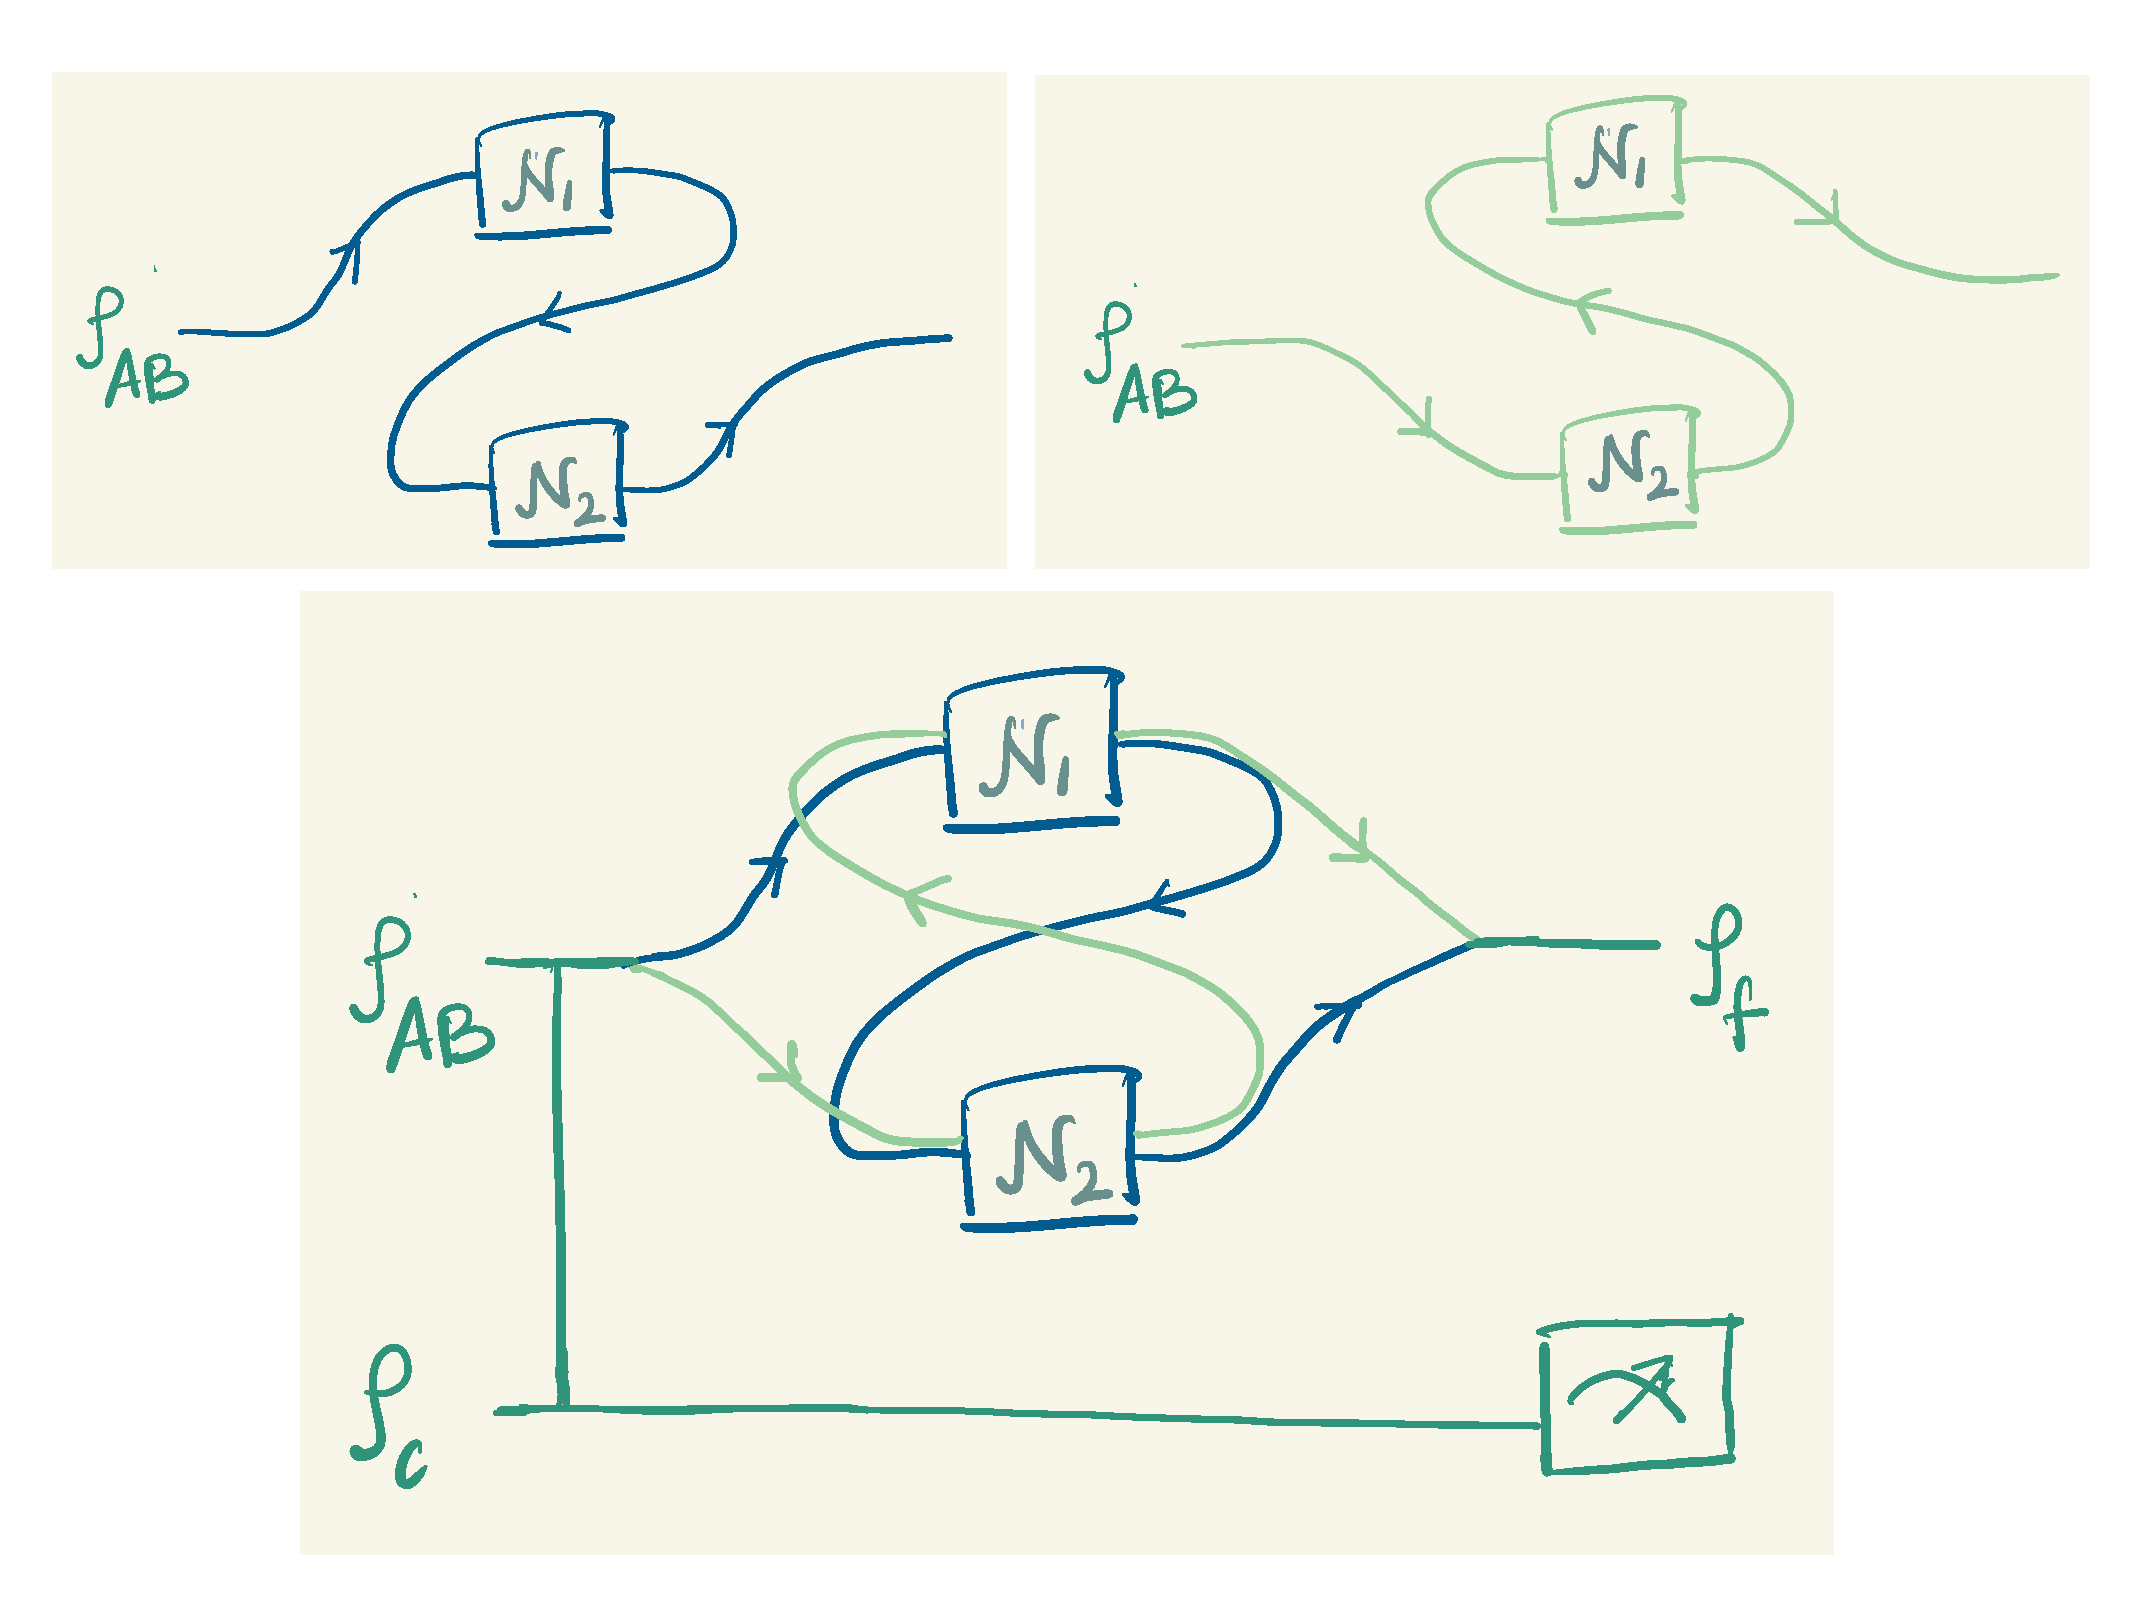
\includegraphics[scale=0.22]{switch_handdrawn_pic.pdf}}
    \caption{\footnotesize{Action of switch.}}
    \label{LHS_eval_cond_modW}
    \end{figure}
\fi

In our case, the two channels under consideration are two global unitary matrices acting on the bipartite system. Let the unitary matrices be $\mathcal{U}_1$ and $\mathcal{U}_2$ and hence the action of the switch can be simplified as given in the following.\\
\textit{The final state of the system after the measurement, considering both the control qubit and the projective measurement on the control qubit in the $\ket{+}$ basis becomes,
\begin{equation}
    \rho_f=\frac{\mathcal{L}_s \rho_{AB} \mathcal{L}_s^{\dagger}}{ Tr[\mathcal{L}_s \rho_{AB} \mathcal{L}_s^{\dagger}]}
    \label{finalstate_switch}
\end{equation}
where, the switching action of the unitary matrices can be seen as, $\mathcal{L}_s=\frac{1}{2}(\mathcal{U}_1 \mathcal{U}_2+\mathcal{U}_2 \mathcal{U}_1)$.}
%\label{prop2}

%\begin{proof}
    \noindent We give a proof of the above statement, particularly for our scenario. We begin by incorporating Eq. (\ref{switchaction}) into Eq. (\ref{FS}) to obtain,
    \begin{equation}
        \rho^{\prime}_{f} =~ _c\bra{+}\sum_{i,j} W_{ij}(\rho_{AB} \otimes \rho_c)W_{ij}^{\dagger}|\ket{+}_c.
    \end{equation}
    Evidently, $\rho_f= \rho^{\prime}_{f}/n$ with $n= Tr [\rho^{\prime}_{f}]$. Let us now simplify the preliminary calculation by considering that the initial state is given by $\rho_c=\ket{+}\bra{+}$. The calculation elaborated in the following is for the case when the control qubit is measured in the $\ket{+}$ state. Hence we have,
    \begin{eqnarray}
        \rho^{\prime}_{f} &=~& _c\bra{+} (\mathcal{U}_1 \mathcal{U}_2 \otimes \ket{0}\bra{0} + \mathcal{U}_2 \mathcal{U}_1 \otimes \ket{1}\bra{1}) \nonumber\\
        &&(\rho_{AB}\otimes \ket{+}\bra{+}) \nonumber\\
        &&(\mathcal{U}^{\dagger}_2 \mathcal{U}^{\dagger}_1 \otimes \ket{0}\bra{0} + \mathcal{U}^{\dagger}_1 \mathcal{U}^{\dagger}_2 \otimes \ket{1}\bra{1}) \ket{+}_c \nonumber\\
        %&=& (\mathcal{U}_1 \mathcal{U}_2 \rho_{AB} \mathcal{U}^{\dagger}_2 \mathcal{U}^{\dagger}_1) \vert \braket{0|+}\vert^4 \nonumber\\
        %&& (\mathcal{U}_1 \mathcal{U}_2 \rho_{AB} \mathcal{U}^{\dagger}_1 \mathcal{U}^{\dagger}_2) \vert \braket{0|+}\vert^2 \vert \braket{1|+}\vert^2 \nonumber\\
        %&& (\mathcal{U}_2 \mathcal{U}_1 \rho_{AB} \mathcal{U}^{\dagger}_2 \mathcal{U}^{\dagger}_1) \vert \braket{0|+}\vert^2 \vert \braket{1|+}\vert^2 \nonumber\\
        %&& (\mathcal{U}_2 \mathcal{U}_1 \rho_{AB} \mathcal{U}^{\dagger}_1 \mathcal{U}^{\dagger}_2) |\braket{1|+}|^4.
        &=& (\mathcal{U}_1 \mathcal{U}_2~|\braket{0|+}|^2 + \mathcal{U}_2 \mathcal{U}_1~|\braket{1|+}|^2 ) \rho_{AB} \nonumber\\
        && (\mathcal{U}^{\dagger}_2 \mathcal{U}^{\dagger}_1~ |\braket{0|+}|^2 + \mathcal{U}^{\dagger}_1 \mathcal{U}^{\dagger}_2~|\braket{1|+}|^2 ) \nonumber\\
        &=& \mathcal{L}_s \rho_{AB} \mathcal{L}^{\dagger}_s, 
    \end{eqnarray}
    with $\mathcal{L}_s=\frac{1}{2}(\mathcal{U}_1 \mathcal{U}_2+\mathcal{U}_2 \mathcal{U}_1)$. Now it is clear that $n=Tr[\mathcal{L}_s \rho_{AB} \mathcal{L}^{\dagger}_s]$ and the final state of the system after the switching action is given by the expression in Eq. (\ref{finalstate_switch}). Hence the claim.\\
The overall effect of switch can be seen by the operator $\mathcal{L}_s$. Note that, this is no more an unitary operation, which enables us to achieve the advantage in our case. 


%--------------------------------------------------------

\chapter{Absolute Separability}
\label{ch:abs}
\section{Separability}
Quantum entanglement is the most powerful resource not only in information processing tasks but also in quantum computation. Here we begin our study in the backdrop of two-qubit systems.
Let $\mathcal{H}^A$, $\mathcal{H}^B$ be Hilbert spaces and let $\ket{\phi} \epsilon$ $\mathcal{H}^A \otimes \mathcal{H}^B$ be a pure state. The state $\ket{\phi}$ is a product state in $\mathcal{H}$ = $\mathcal{H}^A \otimes \mathcal{H}^B$ if there are pure states $\ket{\phi}^A \epsilon \mathcal{H}^A$, $\ket{\phi}^A \epsilon \mathcal{H}^A$ such that 
\begin{equation}
    \ket{\phi} = \ket{\phi}^A \otimes \ket{\phi}^B
\end{equation}
A pure state $\ket{\phi}$ is separable if it is a product state in $\mathcal{H}$. Otherwise the state $\ket{\phi}$ is entangled.
Similarly to pure states, entangled mixed states are the
complement of separable mixed states. However, the definition of
separable states is more complex as it is necessary to differentiate the
definitions of product states and separable states.
Let $\mathcal{H}^A$, $\mathcal{H}^B$ be Hilbert spaces and let $\rho$ be a mixed state over Hilbert space $\mathcal{H}^A \otimes \mathcal{H}^B$, then the state $\rho$ is a product state in $\mathcal{H}$ if there are mixed states $\rho^A \epsilon \mathcal{L}(\mathcal{H^A})$, $\rho^B \epsilon \mathcal{L}(\mathcal{H^B})$ such that
\begin{equation}
    \rho = \rho^A \otimes \rho^B
\end{equation}

Also, for product states ${\rho_i}$ where i=1,2...n, mixed state $\rho \epsilon \mathcal{L}(\mathcal{H})$ is separable if there are convex weights $p_i$>0, $\sum_i p_i = 1$ such that
\begin{equation}
    \rho = \sum_{i=1}^n p_i rho_i
\end{equation}
Also, if a state is not separable, then it is entangled.

 Furthermore, from the definition of separable states, the set of separable states is a convex subset of the set of all mixed states. This leads to the geometrical representation of set of all mixed states as depicted in Figure
2.1. The pure states lie on the edge of the whole set and the set of all
separable states touches the edge of set of all states in infinitely many
points as there is infinitely many separable pure states. The separable
pure states cannot lie on the edge of subset of all separable states as
depicted in Figure 2.1 since they are not convex combinations of any
other states.

\section{Absolute Separable States:}
A quantum state is called absolute separable if any global unitary operation on the state does not result in entanglement. In other words, a bipartite absolute separable states  $\rho_{AB} \in \mathcal{H}_A \otimes \mathcal{H}_B$ is a state such that for all unitary matrices (or even with their successsive applications) $\mathcal{U} : \mathcal{H}_A \otimes \mathcal{H}_B \longrightarrow \mathcal{H}_A \otimes \mathcal{H}_B$, we have $\mathcal{U} \rho_{AB} \mathcal{U}^\dagger \in \mathcal{S}_{asep}$ where, $\mathcal{S}_{asep}$ is the set of all absolute separable states. The set of absolute separable states forms a convex and compact set \cite{GCM_14} and they play the role of free states in the resource theory of non-absolute separability \cite{PMD_22}. In general, it is a difficult task to detect AS states but for qubit-qudit dimension one can have a criterion based on the eigenvalues of the density matrix \cite{Hi_07, S_09, J_13}. In this case, the $2d$ eigenvalues, arranged in a non-increasing order, are $\{\lambda_i^{\downarrow}\}$ with $\sum_i \lambda_i^{\downarrow} =1$. Then a state is AS if and only if the eigenvalues accept the following condition,
\begin{equation}
    \lambda_1^{\downarrow} - \lambda_{2d-1}^{\downarrow} - 2\sqrt{\lambda_{2d-2}^{\downarrow} \lambda_{2d}^{\downarrow}} \leq 0
    \label{AS_eigenvalue}
\end{equation}
The equality of the above equation holds for the states on the boundary of the convex set containing AS states \cite{HMD_21}. From the above inequality, the following consequences emerge immediately. 
\begin{prop}
    In $2\otimes d$ dimension, there exists no AS state with rank $(2d-2)$. \cite{HMD_21}
    \label{prop1}
\end{prop}
\begin{proof}
    The proof of the statement follows from \cite{HMD_21}. Note that, if we have a bipartite state $\rho_{AB}$ with rank $r(\rho_{AB}) \leq (2d-2)$, then we can write the $2d$ number of eigenvalues of the density matrix of $\rho_{AB}$ as, $\{\lambda_1^{\downarrow}, \lambda_2^{\downarrow}, \cdots, \lambda_{2d-2}^{\downarrow}, 0, 0\}$ without any loss of generality (the eigenvalues are arranged in a non-increasing manner). Hence using Eq.(\ref{AS_eigenvalue}), we have the condition on the largest eigenvalue as, $\lambda_1^{\downarrow} \leq 0$, which is not possible. So, one can conclude that there exists no rank $(2d-2)$ AS state in $2\otimes d$ dimension.
\end{proof}
\noindent Now let us consider the case when the rank of the state is $r(\rho_{AB})=(2d-1)$ and the eigenvalues can be written as, $\{\lambda_1^{\downarrow}, \lambda_2^{\downarrow}, \cdots, \lambda_{2d-1}^{\downarrow}, 0\}$. In this case, we have $\lambda_1^{\downarrow} \leq \lambda_{2d-1}^{\downarrow}$ from Eq.(\ref{AS_eigenvalue}). As the eigenvalues are already arranged in non-increasing order, we can set, $\lambda_1^{\downarrow}=\lambda_2^{\downarrow} \cdots= \lambda_{2d-1}^{\downarrow} = \lambda$ (say). Hence, $\lambda=\frac{1}{2d-1}$ as, $\sum_i \lambda_i^{\downarrow} =1$. For example, in a bipartite qubit system, we can have a state $\rho_{AB}=\frac{1}{3} (\ket{00}\bra{00}+\ket{01}\bra{01}+\ket{10}\bra{10})$. Note that from the eigenvalue condition, it is clear that this state resides on the boundary of the convex set in that dimension. At the beginning of our calculation, we consider such types of states and see the action of switching unitary on them. 

%--------------------------------------------------------
\chapter{Using Quantum Switch on AS states}
\label{ch:ch5}
\section{Rank 3 States}
In this section, we discuss the results of ``breaking" absolute separability via quantum switch. Here, by ``breaking" we mean having a separable state from a AS state via global unitary. We start by considering a very simple case to see if it is at all possible. In a bipartite qubit system, let us consider an AS state. Note that, the rank of the state can either be $3$ or $4$. 
    Let us consider a rank $3$ AS state $\rho_{AB}=\frac{1}{3} (\ket{00}\bra{00}+\ket{01}\bra{01}+\ket{10}\bra{10})$ which lies on the boundary of the convex set in $2\otimes 2$ dimension. Under the switching action of two global unitaries, one being CNOT gate and the other given by, 
    \begin{equation}
        U = 
    \begin{pmatrix}
        cos\theta & 0 & 0 & sin\theta\\
        0 & cos\theta & sin\theta & 0\\
        0 & sin\theta & -cos\theta & 0\\
        sin\theta & 0 & 0 & -cos\theta
    \end{pmatrix},
    \label{unitary_theta}
    \end{equation}
    the resulting state is not an AS state.    We know that the CNOT gate in the computational basis is described by,
    \begin{equation}
    V_{CNOT}= \left(
    \begin{array}{cccc}
     1 & 0 & 0 & 0 \\
     0 & 1 & 0 & 0 \\
     0 & 0 & 0 & 1 \\
     0 & 0 & 1 & 0 \\
    \end{array}
    \right)
    \end{equation}
    Now, following Eq.(\ref{finalstate_switch}) with the initial state as $\rho_{AB}$, one can obtain the final state where $\mathcal{U}_1$ and $\mathcal{U}_2$ are CNOT and $U$. The eigenvalues of the final state, arranged in a non-increasing manner are given by, $\{ \frac{4}{3(3+cos2\theta)}, \frac{1}{3}, \frac{2(1+cos2\theta)}{3(3+cos2\theta)},0 \}$. Let us consider the final state obtained is also an AS state. Hence with the given set of eigenvalues, we construct the criterion to identify AS states. Note that, with these eigenvalues, the inequality in Eq. (\ref{AS_eigenvalue}) reduces to $\cos{(2\theta)}\geq 1$, which is itself contradictory. So our assumption is not correct and it implies that the final state is residing outside the set of AS states in the given dimension. Now with PPT criterion, we verify that the state is a separable state. Hence we obtain a separable state starting from an AS state.
\section{Werner States}
Werner formulated mixed state entanglement in a mathematically rigorous framework
and discovered that there are quantum states which exhibit entanglement but no nonlocality [13],
that is, while any separable state can be modeled by a hidden-variable theory and hence satisfies all
generalized Bell inequalities, the converse is not true. This was achieved by a class of quantum states
introduced by Werner in an ingenious way, and now named after him [13]. Since then, the Werner
states, due to their fundamental characteristics and nice features, have been extensively studied and
widely used in quantum information [14–46]. Despite their seemingly simple structure, the Werner
states and their various generalizations exhibit very rich correlations, ranging from separability to
entanglement, from steering to nonlocality, depending on the single intrinsic parameter in the Werner states [31]. Quantitative knowledge and precise engineering of the two-qubit Werner states have rendered these states as a paradigm for both theoretical and experimental explorations of quantum
information. The Werner states (which are mixed in general), together with the Bell states (which
are pure), constitute a popular playground in studying quantum correlations.
Apart from the Bell states, the Werner states are the most prominent examples of bipartite states
and offer a unique testing ground for quantum information investigations. The Werner states on a
bipartite system Hilbert space $\mathcal{H} \otimes \mathcal{H}$ with dim$\mathcal{H}$ = d have at least three representations [13]:
(1) Werner states as linear combination of the identity operator and the swap operator. In this
representation, the Werner states are defined as
\begin{equation*}
    w=\frac{d-x}{d^3-d}\mathbf{I}\otimes\mathbf{I} + \frac{dx-1}{d^3-d}F,\hspace{1cm} x \epsilon [-1,1]
\end{equation*}
where 1 is the identity operator on H, and F is the swap operator on H $\otimes$ H defined as 
\begin{equation*}
    F(\ket{\psi} \otimes \ket{\psi}) = \ket{\psi} \otimes \ket{\psi}, \hspace{1cm} \forall \ket{\psi}, \ket{\psi} \epsilon \mathcal{H}    
\end{equation*}
Explicitly,
\begin{equation*}
    F = \sum^{d}_{\mu,\nu=1} \ket{\mu}\bra{\nu} \otimes \ket{\nu}\bra{\mu},
\end{equation*}
which is independent of the choice of the orthonormal basis {$\ket{\mu}$ : $\mu$ = 1, 2, · · · , d} of H. Clearly,



\subsection{Modified Werner States}
The modified Werner state \cite{W_89} can be written as, 
\begin{equation}
    \rho_W = p \ket{\xi}\bra{\xi}+ \frac{1-p}{4} \mathcal{I}_{4 \times 4}
    \label{mod_Wstate}
\end{equation}
where $\ket{\xi}$ being a pure state of the form, $\ket{\xi} = \cos{\gamma}\ket{00} + e^{i\phi} \sin{\gamma}\ket{11}$, with $0 \leq p \leq 1$, $0 \leq \gamma \leq \pi$ and $0 \leq \phi \leq 2\pi$. It is already well established that the state in Eq. (\ref{mod_Wstate}) is AS for the range $0\leq p \leq \frac{1}{3}$ and it is separable in the region $\frac{1}{3}\leq p\leq \frac{1}{1+2\sin{2 \gamma}}$. Next we move a step further and show that it is possible to achieve separability for a larger region of $p$ when subjected to a global unitary channel via switching order. 
    
\begin{result}
    If the initial state is $\rho_W$ given in Eq.(\ref{mod_Wstate}) and it undergoes the switching operation between two unitary channels, one being CNOT and the other given in Eq. (\ref{unitary_theta}), then it is possible to achieve separability from the region of AS states.
\end{result}

\begin{figure}[htp]
\centering
\fbox{
\subfigure[The eigenvalues of the final state after the switching action on the state in Eq. (\ref{mod_Wstate}) are plotted against the global unitary parameter, $\theta$. Here we consider $p=0.15$ for which  the initial state is AS.]{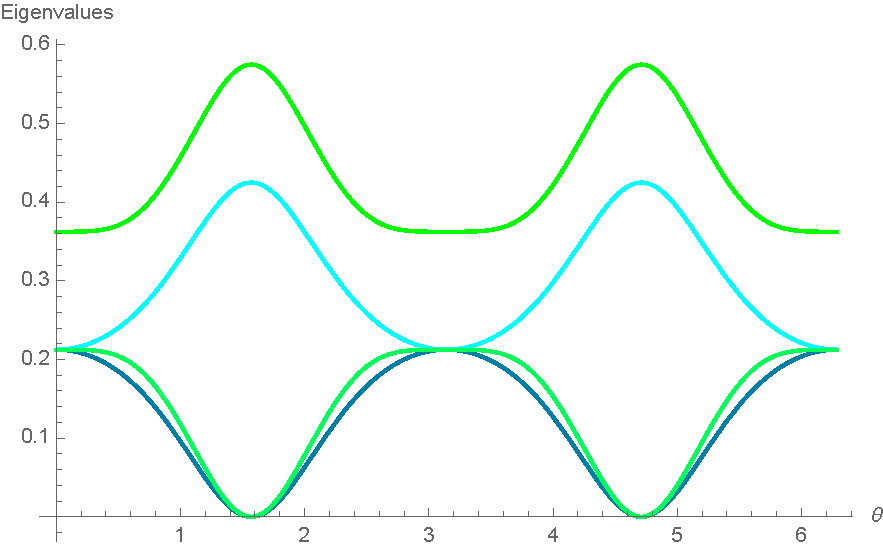
\includegraphics[scale=0.5]{figures/Eigenvalues_modW_f.pdf}}
%\hfill
\qquad
\subfigure[The same eigenvalues are plotted against the noise mixing parameter $p$ ($p$ is varying in the range of AS states) for a fixed $\theta = 1.2$. ]{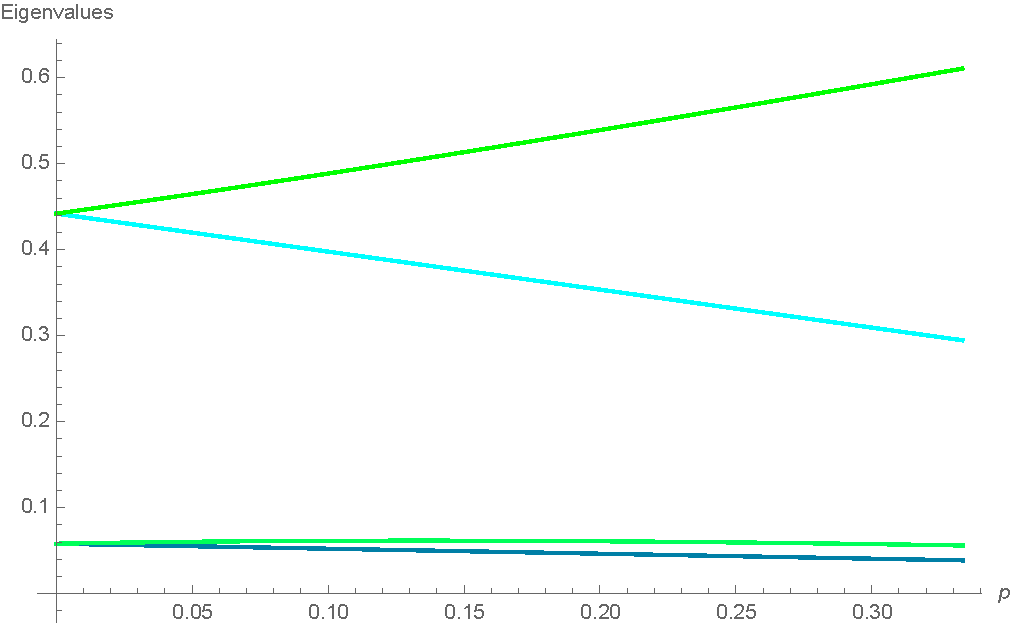
\includegraphics[scale=0.44]{figures/Eigenvalues_modW_f_p.pdf}}}
\caption{\footnotesize{The eigenvalues of the final state}}
\label{eigenvalues_modW}
\end{figure}

    

   \noindent  To prove the statement, we only need to demonstrate an example in which the stated transformation is possible. To begin the demonstration, we observe that the eigenvalues of the initial state in Eq. (\ref{mod_Wstate}) are given by $\{ \frac{1+3p}{4}, \frac{1-p}{4},\frac{1-p}{4},\frac{1-p}{4} \}$, arranged in the non-increasing order. Note that, the eigenvalues are independent of the entanglement content of the pure state $\ket{\xi}$. Now using the process prescribed via Eq. (\ref{finalstate_switch}) with $\mathcal{U}_1=U$ given in Eq. (\ref{unitary_theta}) and $\mathcal{U}_2=CNOT$, we get the eigenvalues of the final state as shown in the Fig. (\ref{eigenvalues_modW}). The eigenvalues are then arranged in non-increasing order for the whole range of the noise mixing parameter $p$ of the state and the unitary matrix parameter $\theta$. 
    
    \begin{figure}[htp]
    \fbox{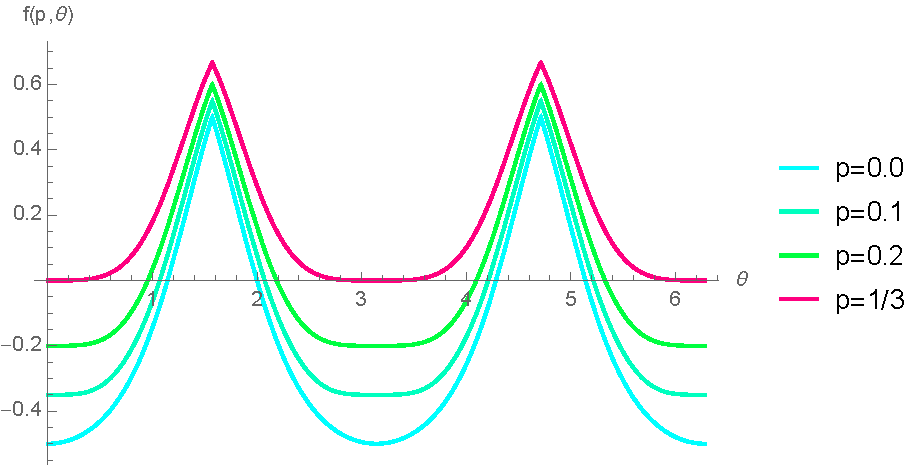
\includegraphics[scale=1]{figures/LHS_eval_cond_modW.pdf}}
    \caption{\footnotesize{The LHS of the eigenvalue condition given in Eq. (\ref{AS_eigenvalue}) is plotted against the unitary matrix parameter for different values of state parameter of AS states.}}
    \label{LHS_eval_cond_modW}
    \end{figure}
    
    In the next step, to check whether the final state remains an AS or not we further evaluate the LHS of Eq. (\ref{AS_eigenvalue}) and obtain the expression as a function of $p$ and $\theta$ (say, $f(p, \theta)$). Plotting this function shows that the condition given in Eq. (\ref{AS_eigenvalue}) is not satisfied for a broad range of $p$ as well as $\theta$ as shown in Fig (\ref{LHS_eval_cond_modW}). Hence for a given choice of unitary it is possible to extend the range of $p$ for which the AS states become separable.
  
   
After proving that it is evidently possible to break absolute separability of modified Werner state via global unitary matrices while employing them with switching order, we look at the results a little bit more carefully. From Fig. (\ref{LHS_eval_cond_modW}) it is clear that for all the values of noise mixing parameter $p$ of the state, there exists certain type of global unitary (corresponding to given values of $\theta$ of $U$ given in Eq. (\ref{unitary_theta})) along with a CNOT gate, which can take out the AS state out of the convex set. Now, looking at Fig (\ref{eigenvalues_modW}.(a)) we see that out of four eigenvalues of the final states, when one becomes $0$ for any value of $p$, another one also goes to $0$. At the same time, the highest eigenvalue takes the largest value. This might happen for several unitary matrices, one being $\theta=\pi/2$ in $U$. Correspondingly, the violation of Eq. (\ref{AS_eigenvalue}) becomes nothing but the largest eigenvalue. For $\theta=\pi/2$, the largest eigenvalue becomes $(1+p)/2$. Note that, the violation hence behaves as a monotonically increasing function of the noise mixing parameter $p$. Interesting even for $p=0$, when the corresponding initial state is a maximally mixed state, it is possible to have the condition for absolute separability violated for certain $\theta$. We emphasise here on the fact that the maximally mixed state $\mathcal{I}/4$ (in $2\otimes2$), which is a free state in every resource theory, it is possible to make it a separable state if one has access to global unitary operations making the initial state resourceful. On the other hand for $p=1/3$, the modified Werner states lie in the boundary of AS states, on the verge of becoming separable. Hence, intuitively it can be assumed that these are the states that are the easiest to take out from the set of convex states containing the AS states. Our result confirms the same as it can be seen from the plot in Fig. (\ref{LHS_eval_cond_modW}) that the choice of effective unitary is extensively high. 
%({\color{red}mention something about rank??!!!})

\begin{figure}[htp]
\centering
\fbox{
\subfigure[For $p=0$ (maximally mixed state)]{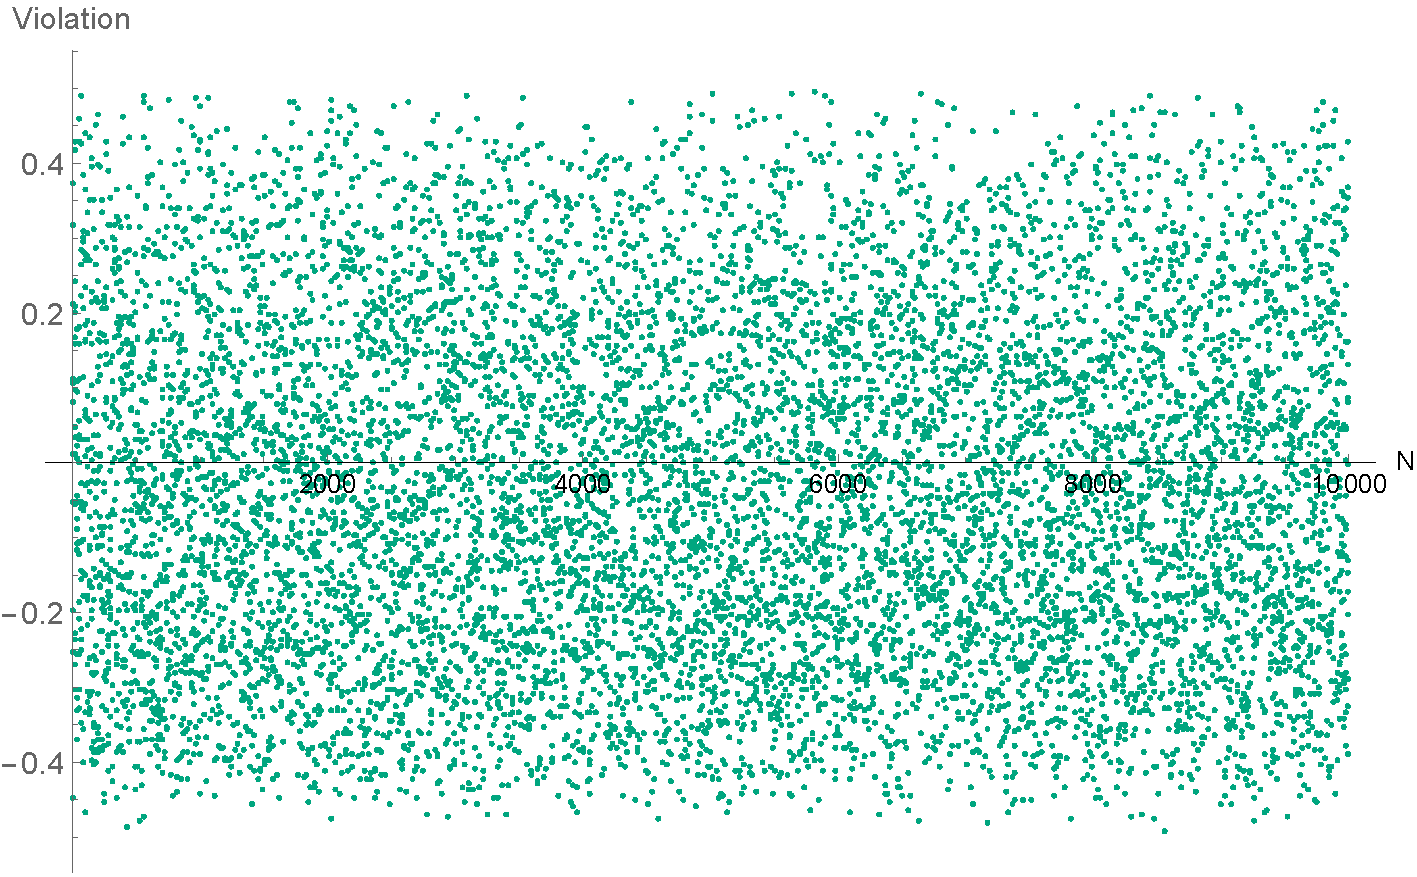
\includegraphics[scale=0.3]{figures/RandomU_p0_10k.pdf}}
%\hfill
\qquad
\subfigure[For $p=1/3$, $\phi=0$, and $\gamma=\pi/4$]{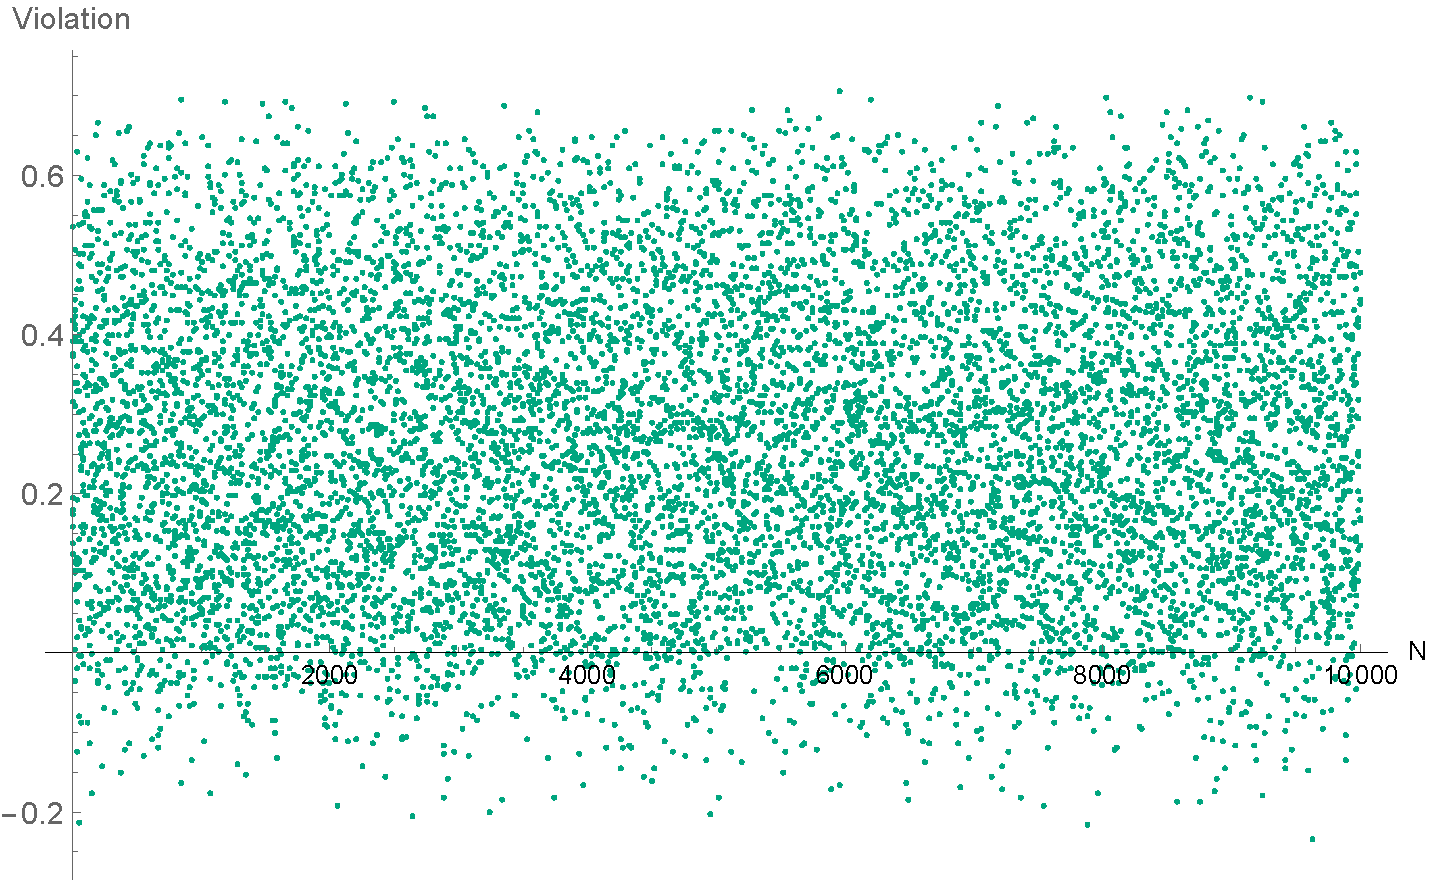
\includegraphics[scale=0.3]{figures/RandomU_p1_3_10k.pdf}}}
\caption{\footnotesize{We plot the LHS of Eq.(\ref{AS_eigenvalue}) for $2\otimes2$ dimension (Violation) against the number of  Haar uniformly generated random unitary matrices (N) for two choices of noise mixing parameter $p$ for modified Werner state.}}
\label{RandomU_modW}
\end{figure}

Now to generalise our result numerically by considering that we have access to one CNOT gate and the other unitary is made completely random. We generate random $100000$ unitary matrices Haar uniformly. Here, we consider two cases corresponding to two initial states, (a) maximally mixed state in $2\otimes2$ dimension i.e. $p=0$ in Eq. (\ref{mod_Wstate}), and (b) $p=1/3$, $\phi=0$, and $\gamma=\pi/4$ in Eq. (\ref{mod_Wstate}), giving us a mixture of white noise with maximally entangled state in $2\otimes2$. For illustration, we plot the cases for $10000$ randomly generated unitary matrices in Fig.(\ref{RandomU_modW}). Note that, both the plots evidently show that it is always possible to find a global unitary operation that makes a AS state a separable one by switching operation with CNOT gate. As can be guessed intuitively, the number of useful unitary matrices to break absolute separability, for Case (b) is more than that for in Case (a) as the state in Case (b) is lying on the boundary of the convex set. We extend our result to higher dimension ($2\otimes d$) by considering maximally mixed state initially while both the random unitary matrices are generated Haar uniformly. We check the absolute separability criterion given in Eq. (\ref{AS_eigenvalue}) and plot the violation. The plots with more details can be found in the appendix.\\
Another interesting observation that can be made from the results of switching action on modified Werner state is about the rank of the final state. The initial state given in Eq. (\ref{mod_Wstate}) is a full-rank state for the whole range of noise mixing parameter $p$. After the switching action, the rank of the final state remains unaltered in most of the cases except for $\theta=\pi/2$ and for odd multiples of $\pi/2$. In these exceptional cases the rank decreases to 2 and making the final state certainly separable as can be seen from Proposition (\ref{prop1}). At the same time, from numerical simulation we find that rank remains unchanged for all the cases. 

\section{Bell diagonal states}

\begin{figure*}[htp]
\centering
\fbox{
\subfigure[Structure of Bell Diagonal states. The octahedron represents the set of separable states \cite{LC_10}, and the inner structure represents the AS states.]{\includegraphics[scale=0.3]{figures/BDstate_AS_Sep_2.pdf}}
%\hfill
\qquad
\subfigure[Structure of BD AS states after switching action for Unitary corresponding to $\theta=\pi/6$]{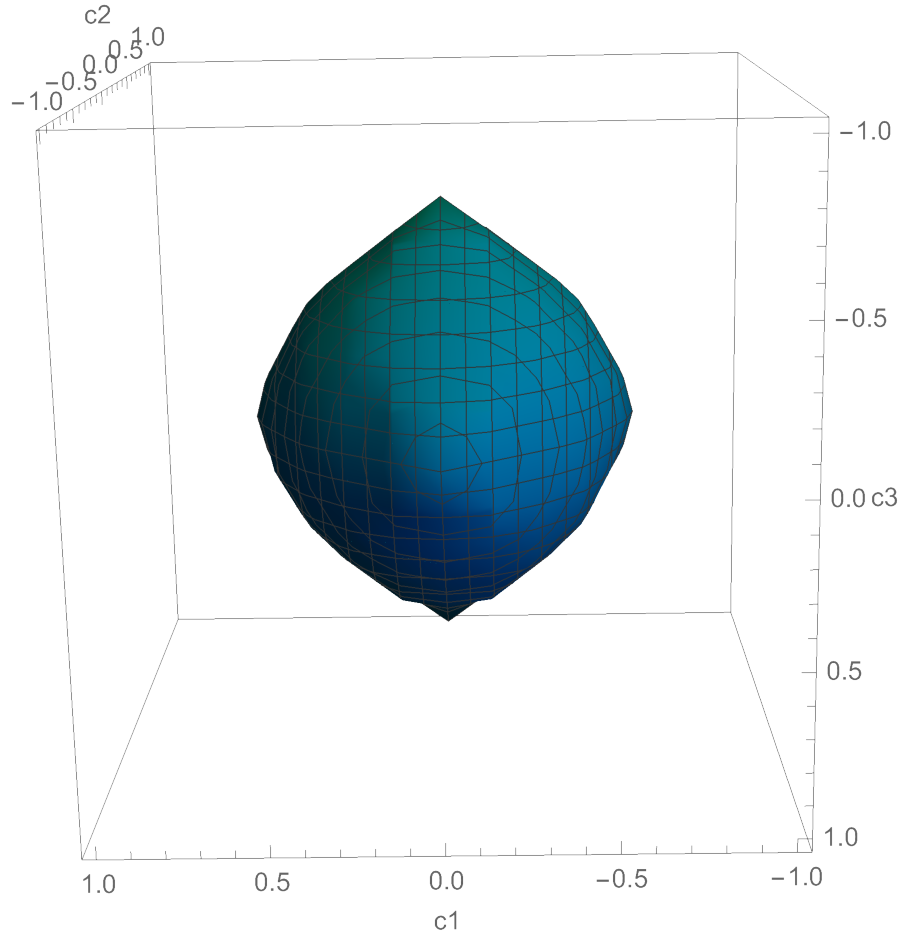
\includegraphics[scale=0.2]{figures/BD_switch_pi_6.pdf}}
\qquad
\subfigure[Structure of BD AS states after switching action for Unitary corresponding to $\theta=\pi/4$]{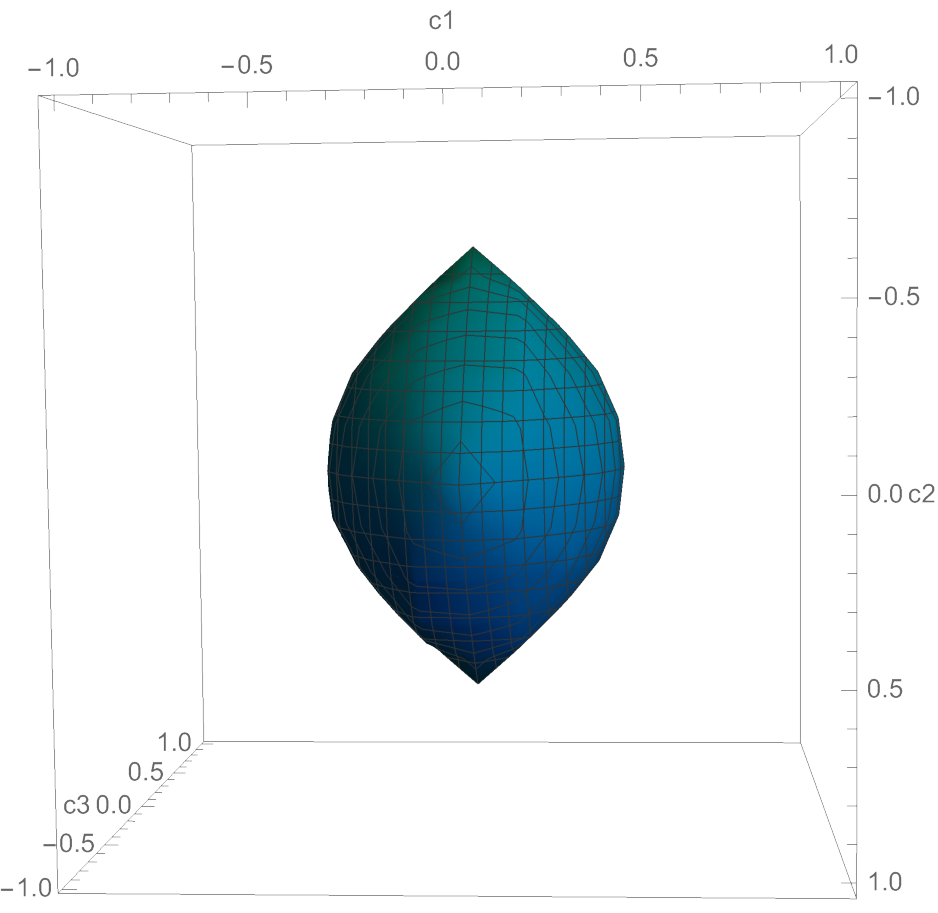
\includegraphics[scale=0.2]{figures/BD_switch_pi_4.pdf}}
\qquad
\subfigure[Structure of BD AS states after switching action for Unitary corresponding to $\theta=\pi/3$]{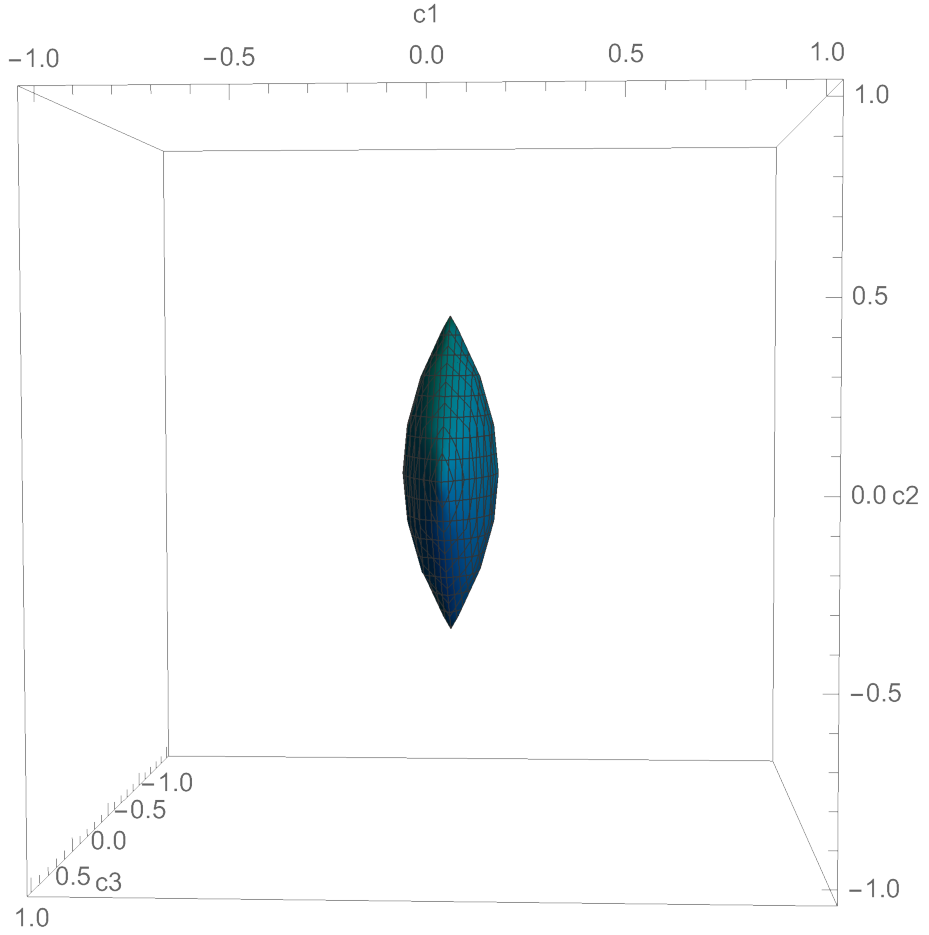
\includegraphics[scale=0.2]{figures/BD_switch_pi_3.pdf}}
}
\caption{\footnotesize{Geometry of BD AS states before and after switching action of global unitary matrices.}}
\label{BD_AS_sep_switch}
\end{figure*}

   % \fbox{\includegraphics[scale=2*0.45]{BDstate_AS_Sep_2.pdf}}
   % \caption{\footnotesize{Structure of Bell Diagonal states. The bigger tetrahedron represents the set of separable states [ref], and the inner structure represents the AS states.}}


Next we move our discussion to the set of Bell-diagonal (BD) states. For that, we first introduce and elaborate the properties of this particular state in the following. The two-qubit Bell diagonal states are the probabilistic mixture of maximally entangled states given in the following form,
\begin{eqnarray}
    \rho_{BD} &=& p_1 \ket{\phi^+}\bra{\phi^+} + p_2 \ket{\phi^-}\bra{\phi^-} + p_3 \ket{\psi^+}\bra{\psi^+} \nonumber \\
    && + p_4 \ket{\psi^-}\bra{\psi^-}
    \label{BD_state_p}
\end{eqnarray}
with, $p_1+p_2+p_3+p_4=1$. Here, $\ket{\phi^{\pm}}=(\ket{00}\pm \ket{11})/\sqrt{2}$ and $\ket{\psi^{\pm}}=(\ket{01}\pm \ket{10})/\sqrt{2}$ are four Bell states. In the Bell-basis, this is a diagonal state. From the partial transposition criterion, it is evident that $\rho_{BD}$ is a separable state if all the mixing probabilities are less than or equal to $1/2$. Note that, the eigenvalues of the state in Eq. (\ref{BD_state_p}) are given by, $\{ p_1, p_2, p_3, p_4\}$. Another form of the state is \cite{LC_10},
\begin{equation}
    \rho_{BD} = \frac{1}{4} (\mathcal{I}+\sum_{i=1}^3 c_i \sigma_i \otimes \sigma_i)
    \label{BD_state_c}
\end{equation}
with $\sigma_i$'s being the Pauli matrices.

\noindent Comparing equations (\ref{BD_state_p}) and (\ref{BD_state_c}), one can get the constraints on the coefficients $c_1$, $c_2$ and $c_3$ which eventually indicates the region describing the separable states and the AS states \cite{LC_10}. For the state to be separable, we have $|c_1|+|c_2|+|c_3| \leq 1$ which gives a tetrahedron structure as illustrated in Fig. (\ref{BD_AS_sep_switch} (a)). Explicitly, $p_1=(1+c_1-c_2+c_3)/4$, $p_2=(1+c_1+c_2-c_3)/4$, $p_3=(1-c_1+c_2+c_3)/4$ and $p_4=(1-c_1-c_2-c_3)/4$. Putting the eigenvalue condition (\ref{AS_eigenvalue}) on these mixing parameters along with the condition of positivity, we find the conditions on $c_1$, $c_2$ and $c_3$ for $\rho_{BD}$ to be an AS state which enables us to obtain the structure of AS states as also illustrated in Fig. (\ref{BD_AS_sep_switch} (a)). 
\begin{result}
    If the initial state is $\rho_{BD}$ given in Eq.(\ref{BD_state_c}) and it undergoes the switching operation between two unitary channels, one being CNOT and the other given in Eq. (\ref{unitary_theta}), then it is possible to change the structure of the set of AS BD states for varying the parameter $\theta$ in Eq. (\ref{unitary_theta}) as shown in Fig. (\ref{BD_AS_sep_switch} (b), (c), (d)). 
\end{result}
For the understanding of the result we refer to Fig. (\ref{BD_AS_sep_switch}). Let us now note some observations that can be made from the mentioned figure. Firstly, the size of the set of AS BD states decreases with the increasing $\theta$ value. Eventually, it can been seen for $\theta=\pi/2$ the set completely vanishes which implies that all the BD AS states can be made atleast separable under suitable choice of global unitary matrices.

\begin{figure*}[htp]
\centering
\fbox{
\subfigure[BD states for $\alpha=0.17$ to $0.5$. Here, $N=(\alpha-0.17)/0.01$.]{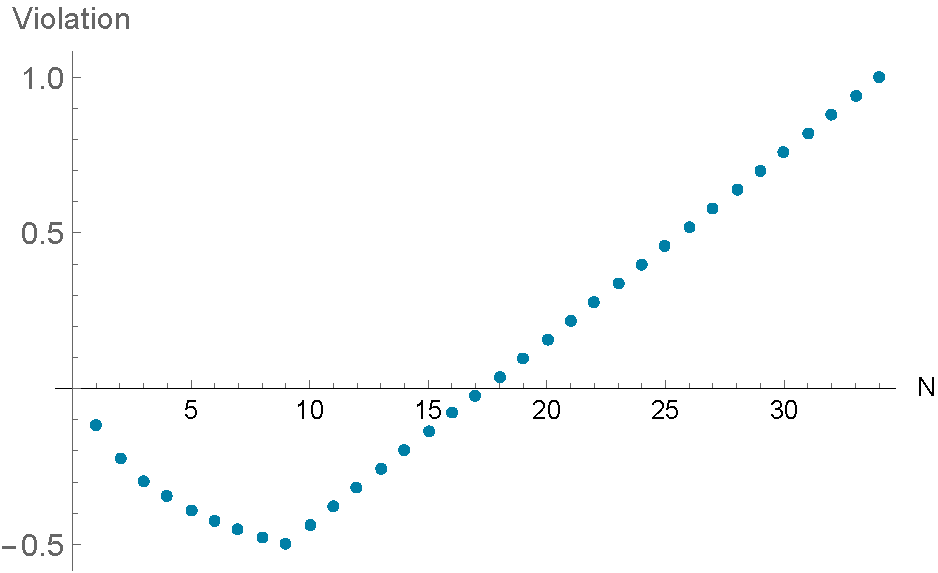
\includegraphics[scale=0.22]{figures/BD_3_alpha_vio.pdf}}
%\hfill
\qquad
\subfigure[For $\alpha=0.18$ after Switching action. (Here, $N$ is number of random unitary.)]{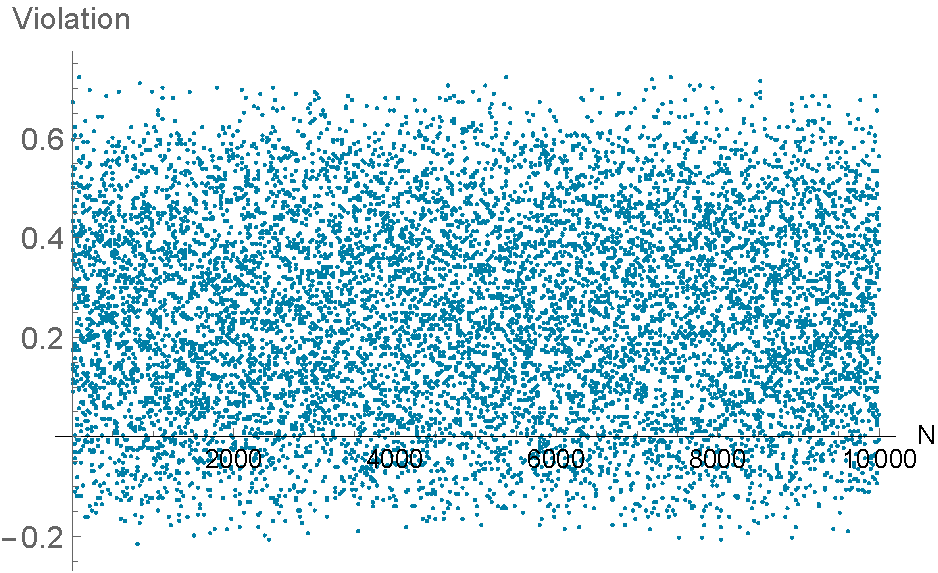
\includegraphics[scale=0.22]{figures/BD_3_alpha_0.18_switch.pdf}}
\qquad
\subfigure[For $\alpha=0.20$ after Switching action. (Here, $N$ is number of random unitary.)]{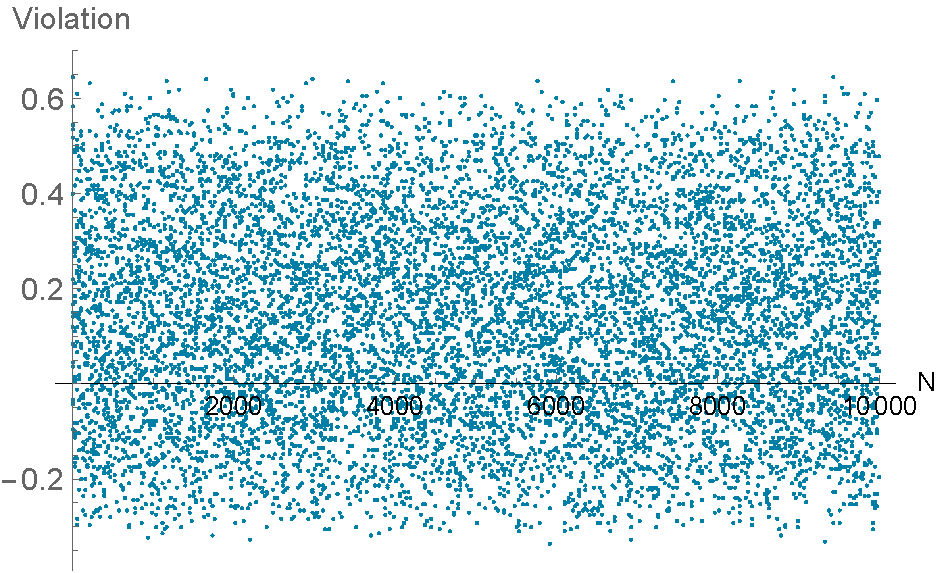
\includegraphics[scale=0.22]{figures/BD_3_alpha_0.2_switch.pdf}}
\qquad
\subfigure[For $\alpha=0.26$ after Switching action. (Here, $N$ is number of random unitary.)]{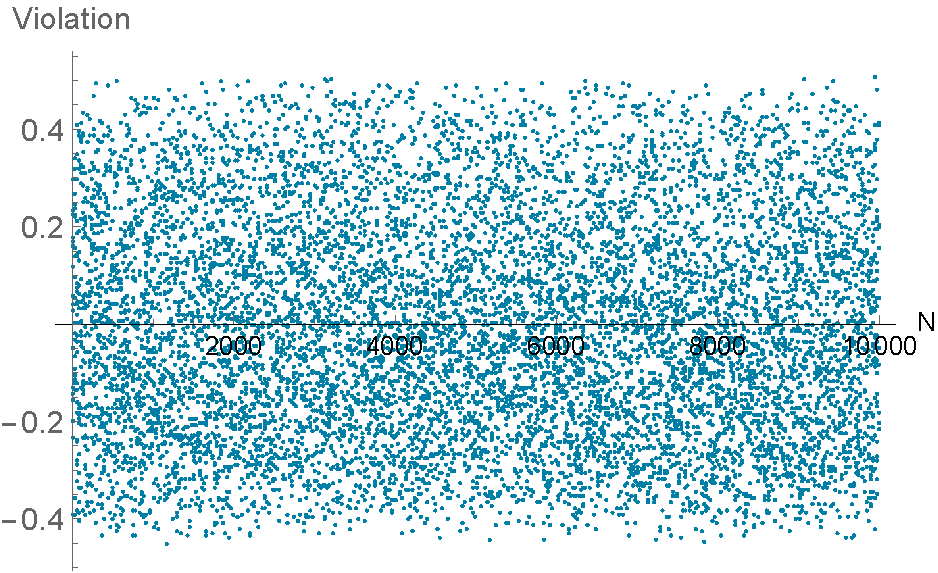
\includegraphics[scale=0.22]{figures/BD_3_alpha_0.26_switch.pdf}}}
\caption{\footnotesize{A particular type of BD state and Switching action of random unitary and CNOT gate on them.}}
\label{BD_random}
\end{figure*}

Now let us consider a particular case of BD state. We choose, three of the mixing parameter having the same value i.e. $p_2=p_3=p_4=\frac{1}{2}-\alpha$ making, $p_1=3\alpha-1/2$ with $\alpha$ running from $1/6$ to $1/2$. In this case, we plot the eigenvalue condition given in Eq. (\ref{AS_eigenvalue}) to find the range for AS states as shown in Fig. (\ref{BD_random}(a)). Then for some particularly chosen values of $\alpha$ we take CNOT gate along with a randomly generated unitary (Haar uniformly generated) and check the switching action on the given state as shown in Fig. (\ref{BD_random} (b), (c), (d)). It is clear from the plots that as $\alpha$ increases, the number of effective unitary matrices (though there always exists many) decreases. It is intuitive as from plot (a) in Fig. (\ref{BD_random}) the lower values of $\alpha$ are nearer to the boundary of the set of AS states. 


%\textcolor{blue}{If possible please workout this as a toy example with the help of fixed $U$ and $\alpha$ by calculating the condition.}



\section*{Results on higher dimensions}
\noindent  For the dimensions $2\otimes d$ we consider the maximally mixed state i.e. $\mathcal{I}_{2\otimes d}/2d$ as the initial state. This is definitely AS and moreover this is a free state in every resource theory. Then we Haar uniformly generate two unitary matrices and use them in switching action on the initial state. We explicitely deal with three cases of dimensions $2\otimes 3$, $2 \otimes 4$, and $2 \otimes 10$. The cases are plotted in Fig. (\ref{higher_d}). From the figure, it is evident that even in higher dimension where the condition given in Eq. (\ref{AS_eigenvalue}) holds, it is possible to find numerous number of global unitary matrices which can make AS states resourceful. Note that, the criterion stated in Eq. (\ref{finalstate_switch}) remains unchanged in these cases. 

\begin{figure*}[htp]
\centering
\fbox{
\subfigure[For $2\otimes 3$ dimension.]{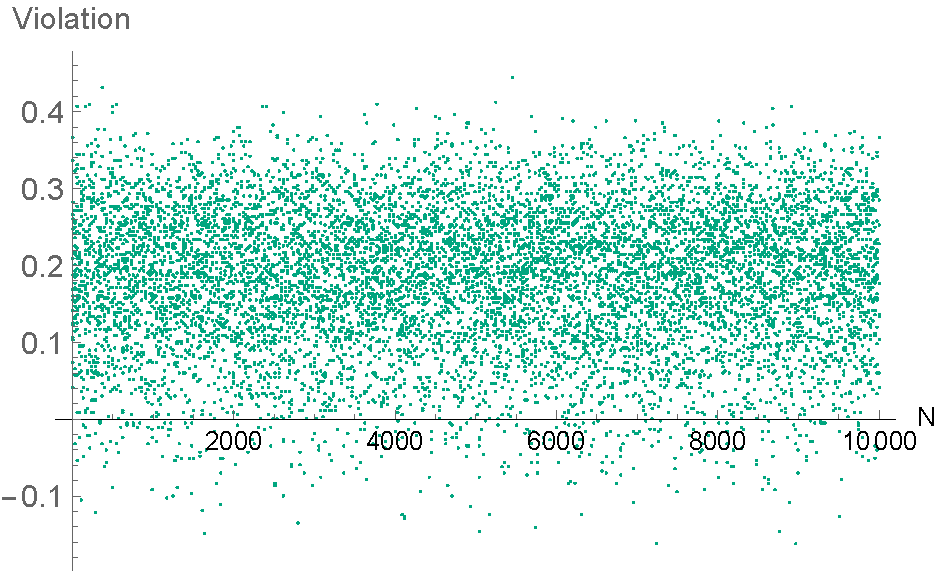
\includegraphics[scale=0.32]{figures/RandomU_2_3.pdf}}
%\hfill
\qquad
\subfigure[For $2\otimes 4$ dimension.]{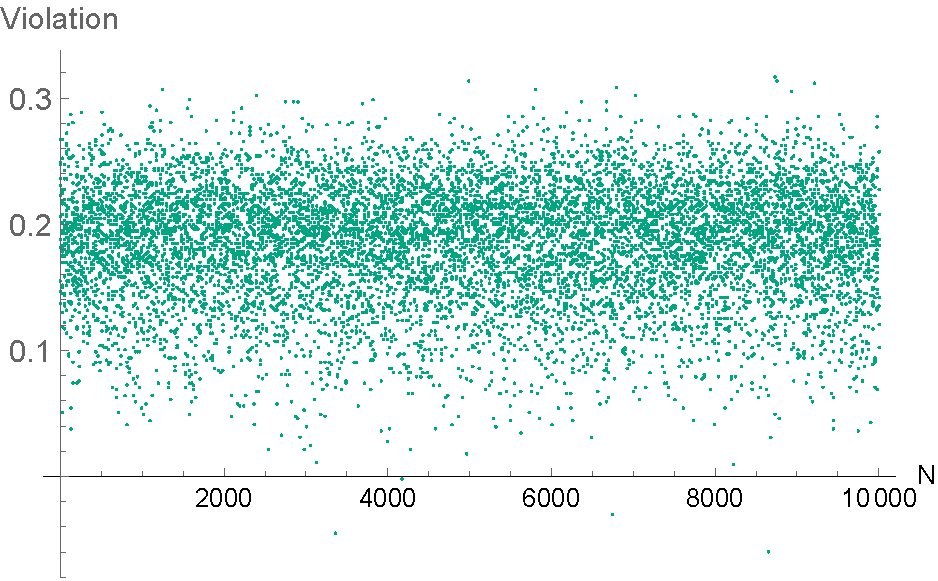
\includegraphics[scale=0.32]{figures/RandomU_2_4.pdf}}
\qquad
\subfigure[For $2\otimes 10$ dimension.]{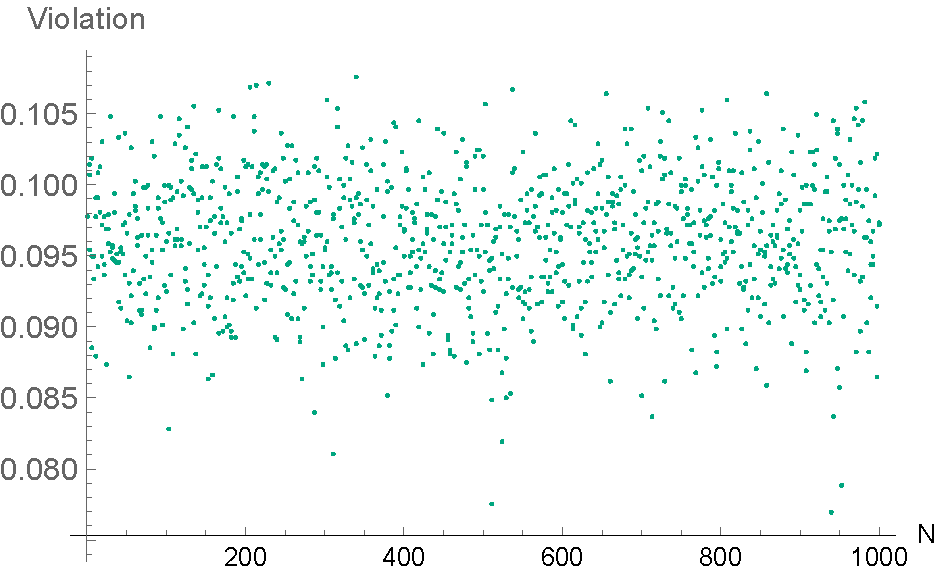
\includegraphics[scale=0.32]{figures/RandomU_2_10.pdf}}}
\caption{\footnotesize{Breaking absolute separability in higher dimensions. The axes have their usual meaning.}}
\label{higher_d}
\end{figure*}



%--------------------------------------------------------

%\chapter{Conclusion}
%\label{ch:conc}
%\input{sections/conclusion.tex}

%--------------------------------------------------------
\bibliographystyle{IEEEtran}
\bibliography{IEEEabrv,cite.bib}{}

% %--------------------------------------------------------
% % 'Publication 1'
% \chapter*{Publications}
% \chapter*{Publication 1}
% \addtocontents{toc}{\protect{\addvspace{3.0ex plus 1pt}}}
% \addcontentsline{toc}{chapter}{\protect{Publication 1}}
% \input{sections/paper1.tex}
% \includepdf[pages={-}]{papers/paper1.pdf}
% %
% %--------------------------------------------------------
% % 'Publication 2'
% \chapter*{Publication 2}
% \addtocontents{toc}{\protect{\addvspace{3.0ex plus 1pt}}}
% \addcontentsline{toc}{chapter}{\protect{Publication 2}}
% \input{sections/paper2.tex}
% \includepdf[pages={-}]{papers/paper2.pdf}

\end{document}
